%% Paper A: what matters in spatial indexing of large point clouds.
%% Elsevier CAS double-column class (cas-dc), for Computers & Graphics.
%% Sections live in sections/*.tex; every number in the results comes from the macros in
%% generated/numbers.tex, written by scripts/paper/macros.py from results/eval_traces. Tables are
%% generated/tab_*.tex and figures are figures/fig_*.pdf, from scripts/paper/tables.py and figures.py.
%% The previous manuscript (2026-08, opposite thesis, pre-rewrite numbers) is kept under old/.
\documentclass[a4paper,fleqn]{cas-dc}

\usepackage[numbers]{natbib}
\usepackage{amsmath}
\usepackage{amssymb}
\usepackage{booktabs}
\usepackage{multirow}
\usepackage{enumitem}
\usepackage{tikz}
\usetikzlibrary{positioning,arrows.meta,fit,backgrounds,calc,shapes.geometric}
\usepackage{placeins}  % \FloatBarrier keeps the results' figures inside the results
% NOTE: cas-dc loads hyperref and graphicx itself; loading them again causes an option clash.

% Double-anonymized review: \anonymoustrue removes the authors, affiliations, acknowledgements and
% funding, and the text refers to the earlier nested-structures paper in the third person throughout.
\newif\ifanonymous
\anonymoustrue

% Diagram palette shared with the generated figures (scripts/paper/figures.py uses the same values).
\definecolor{mdsink}{gray}{0.25}
\definecolor{mdsline}{gray}{0.45}
\definecolor{mdsfill}{gray}{0.94}
\definecolor{mdsaccent}{RGB}{0,90,150}
\definecolor{mdsaccentfill}{RGB}{224,238,247}
\definecolor{mdsout}{RGB}{150,75,0}
\definecolor{mdsoutfill}{RGB}{250,235,215}
\tikzset{
  mdsbox/.style={draw=mdsline, fill=mdsfill, rounded corners=1.5pt, align=center,
                 font=\scriptsize, inner sep=3pt, minimum height=6.5mm},
  mdsmeasured/.style={mdsbox, draw=mdsaccent, fill=mdsaccentfill},
  mdsartifact/.style={mdsbox, draw=mdsout, fill=mdsoutfill},
  mdsflow/.style={-{Stealth[length=4pt]}, draw=mdsline, thick},
  mdslabel/.style={font=\tiny\itshape, text=mdsink, inner sep=1.5pt},
}

% Measured quantities. generated/numbers.tex defines one macro per number; a missing macro must
% fail the build rather than print a stale value, so there is no fallback definition here.
\InputIfFileExists{generated/numbers}{}{\typeout{generated/numbers.tex missing: run scripts/paper/macros.py}}

% Schema names in the compact notation of Section 3.2 (kd48l128sm, qt6_kd48l128sm, ...).
\newcommand{\schema}[1]{\texttt{#1}}
\newcommand{\us}{\,\textmu s}

% Float placement: the paper has many table* and figure* floats; without these the figures queue up
% behind the tables and land after the references.
\renewcommand{\topfraction}{0.9}
\renewcommand{\dbltopfraction}{0.9}
\renewcommand{\bottomfraction}{0.6}
\renewcommand{\textfraction}{0.07}
\renewcommand{\floatpagefraction}{0.75}
\renewcommand{\dblfloatpagefraction}{0.75}
\setcounter{topnumber}{3}
\setcounter{dbltopnumber}{3}
\setcounter{bottomnumber}{2}
\setcounter{totalnumber}{5}

\begin{document}
\let\WriteBookmarks\relax
\def\floatpagepagefraction{1}
\def\textpagefraction{.001}

\shorttitle{Spatial indexes for large point clouds from RAM to disk}
\ifanonymous
  \shortauthors{Anonymous}
\else
  \shortauthors{L\'opez-Ruiz et~al.}
\fi

\title[mode = title]{Spatial indexes for large point clouds from RAM to disk: primitive, leaf and memory layout}

\ifanonymous
  \author[1]{Anonymous authors}
  \affiliation[1]{organization={Anonymized for review}}
\else
  \author[1]{Alfonso L\'opez-Ruiz}
  \cormark[1]
  \ead{allopezr@ujaen.es}
  \credit{Conceptualization, Methodology, Software, Investigation, Writing -- original draft}
  \affiliation[1]{organization={University of Ja\'en}, country={Spain}}
  \cortext[cor1]{Corresponding author}
\fi

\begin{abstract}
% DRAFT: the out-of-core and multi-threaded sentences are completed when batteries 2v-2x are in.
Point-cloud pipelines issue one neighbourhood query per point per stage, so the spatial index is their inner loop, and the cloud may sit in memory, on a solid-state drive or on a hard disk. We ask what sets query time across that hierarchy when every candidate index is built by one engine, tuned under the same budget and measured on held-out query traces of real pipeline stages. On 73 clouds of 17 scenes from one million to one billion points, choosing the primitive and tuning its leaf account for the whole gain over library defaults (1.66 times over an octree, 1.53 over a median kd-tree), and a single split on a scene's flatness picks the primitive within 4 to 8 percent of a per-cloud search. nanoflann's default already ties the tuned structure from one million to one billion points, while four other libraries are 1.6 to 2.6 times slower by implementation. In memory, a node visit costs 35 ns near the root and 350 ns at a leaf, so node counts do not predict time; two-megabyte pages speed every structure by 4 to 9 percent and move the best leaf, so a leaf recommendation carries its page size. Out of core, on four measured devices, the primitive transfers and the leaf follows the device, from 64 to 128 points in memory to thousands on a drive, and keeping the hierarchy in memory is several times faster than paging it. Composing primitives into nested hierarchies, tested as one more option, never improved on a tuned single structure with the hierarchy in memory. The engine, traces and scripts are released.
\end{abstract}

\begin{highlights}
\item Primitive and leaf give 1.5--1.7x over library defaults; one feature picks them
\item nanoflann's default ties the tuned structure from 1M to 1B points
\item A node visit costs 35--350 ns by depth, so visit counts do not predict time
\item Huge pages speed every structure 4--9\%; the best leaf depends on the page size
\item Out of core the leaf follows the device; keep the hierarchy in memory
\end{highlights}

\begin{keywords}
point clouds \sep spatial indexes \sep kd-tree \sep out-of-core \sep memory hierarchy \sep LiDAR \sep performance evaluation
\end{keywords}

\maketitle

\section{Introduction}\label{sec:introduction}

The spatial queries that dominate point-cloud processing are not the sparse requests of an interactive user but the dense, machine-generated ones of a pipeline: normal estimation asks for the nearest neighbours of every point, outlier removal and clustering ask for the points within a radius of every point, and feature computation does both again at several scales. A cloud of a hundred million points puts hundreds of millions of neighbourhood queries through its index per stage, and surveys of a billion points are now routine. The index is the inner loop of the application, and its choice is a design decision that a practitioner makes once, by habit or by a library's default.

The decision has several parts. The first is the primitive: a kd-tree, an octree, a quadtree, a grid, an R-tree or a bounding-volume hierarchy, each with its own fan-out and its own way of cutting space. The second is the parameters: the leaf capacity, the depth, the split rule. The third is the memory layout: how nodes and points are stored and visited. A fourth part has been proposed repeatedly over the last decade: \emph{composition}, the nesting of several primitives in one hierarchy so that the structure changes with depth, a wide one at the top and a fine one below. Several hybrid indexes for point clouds have been reported to beat single structures~\cite{wang2021hybridpointcloud,park2021nestedoctree,ogayar2023nestedlidar}, among them the nested data structures for LiDAR of Ogayar-Anguita et al.~\cite{ogayar2023nestedlidar}, whose quadtree-over-octree schemas loaded fewer nodes than either structure alone on airborne scans. The evidence for composition has two recurring features: it is measured against single structures at default parameters, and it is counted in nodes visited or loaded rather than in time.

This paper asks a simpler question than the hybrid literature does. When every candidate, single or nested, is built by the same engine into the same memory layout, tuned under the same budget, and measured on the queries a real pipeline issues, held out from the selection, where does the speed come from? And does composition survive that measurement?

To answer it we built an instrument rather than an index: an engine that compiles any composition of primitives into one node pool and one traversal, a grammar of schemas that makes a single structure the one-block case of a nested one, and a search that is free to return either. We ran it on \nCells{} cells of \nScenes{} scenes from one million to one billion points, from terrestrial and mobile scans to airborne surveys and forests, with query traces recorded from three pipeline stages and split into a half the search sees and a half it is judged on. We then took the question out of memory, to seven other workloads, to the GPU, to emulated node costs, and to out-of-core stores with the leaves and then the hierarchy on four classes of device; we timed five external libraries on the same traces under one protocol; and we priced every node visit by depth to see where a query's time goes.

The findings are these.
\begin{itemize}[leftmargin=*, itemsep=2pt]
\item \textbf{The primitive and the leaf are the levers.} Choosing the primitive and tuning its leaf, depth and split rule account for the whole gain between a library default and the best structure a search can find, a factor of \leverOctreeDefaultTuned{} over an octree default and \leverKdDefaultTuned{} over a median kd-tree, at every size from one million to one billion points. Composition adds nothing: the best nested schema is \nestedSingleAll$\times$ the best single over \nCells{} cells, was never selected, and the picture is the same on seven workloads, on the GPU, under emulated node costs, and with the leaves out of core.
\item \textbf{Composition pays only with the hierarchy paged.} A nested prefix is adopted in \oocPagedAdopted{} of \oocPagedCells{} out-of-core cells, all with the hierarchy itself read page by page from a slow device, which is the regime of the 2023 result and accounts for it; pinning the hierarchy, a few tens of megabytes at 100M points, is several times faster than any paged schema.
\item \textbf{One feature picks the primitive.} A single split on a scene's flatness score, kd-tree below and quadtree above, is within \ruleRegret{} to \ruleRegretTimed$\times$ of a per-cloud search, closing \ruleCapturePct\% of the gap from the default; nanoflann's default is already that structure for three-dimensional scenes and ties the tuned pick, while four other libraries are 1.6 to 2.6$\times$ slower by implementation.
\item \textbf{Node counts do not predict time; layout does.} A node visit costs \visitCostTopNs\,ns near the root and \visitCostLeafNs\,ns at a leaf, so the visits a wide prefix saves are the cheap ones, and count-based cost models explain under half of the measured lever. Two-megabyte pages speed every structure by \hugeSinglesHundredM$\times$ at 100M points and up to \hugeMin$\times$ for the largest pools, more than composition ever did, and they move the optimal leaf, so a result measured on 4\,KiB pages carries the page size with it.
\end{itemize}

The paper is a revisit, and we say so: one of its findings reverses a result published by some of the present authors' community, and the mechanism that explains the reversal, untuned baselines and node counts in place of time, is the mechanism of the hybrid-index literature at large. What we offer in its place is smaller and, we think, more useful: a controlled protocol, a released instrument with its traces, configurations and scripts, and a rule a practitioner can apply without a search.

Section~\ref{sec:related} places the work. Section~\ref{sec:instrument} describes the engine, the grammar and the search; Section~\ref{sec:setup} the scenes, workloads, protocol and hardware. Section~\ref{sec:results} reports the levers, composition in and out of memory, the rule, the libraries and the mechanism. Section~\ref{sec:discussion} discusses why hybrids have looked good, what transfers, and what the study does not settle.

\section{Related work}\label{sec:related}

\subsection{Spatial primitives and point-cloud libraries}

Spatial indexing methods decompose geometric space through fundamentally distinct partitioning principles. Data-driven binary space partitioning is exemplified by the kd-tree of Bentley~\cite{bentley1975kdtree}, extended to nearest-neighbor search by Friedman et~al.~\cite{friedman1977kdtree}. In point clouds, the choice of split heuristic alters the geometric properties of the resulting cells: while classical median splits guarantee balanced tree height, they frequently generate elongated, high-aspect-ratio bounding boxes in regions with non-uniform point density. The sliding-midpoint rule of Maneewongvatana and Mount~\cite{maneewongvatana1999sliding} mitigates this degeneration by bounding cell aspect ratios, ensuring that empty or sparse regions do not distort spatial pruning. Conversely, space-driven subdivisions partition coordinate domains into regular geometric cells: the quadtree of Finkel and Bentley~\cite{finkel1974quadtrees} and the octree of Meagher~\cite{meagher1980octree}, surveyed exhaustively by Samet~\cite{samet2006foundations}, use bitwise coordinate interleaving for fast cell location and hierarchical level-of-detail extraction. However, because their subdivision geometry is decoupled from data density, uniform octrees can exhibit deep, sparse branch paths when points lie on thin two-dimensional surfaces or terrain manifolds.

Object-driven bounding volume hierarchies group clusters of geometric entities under tight bounding volumes. Classical spatial database indexes include the R-tree of Guttman~\cite{guttman1984rtree}, the R$^*$-tree of Beckmann et~al.~\cite{beckmann1990rstar}, and the bulk-loaded sort-tile-recursive (STR) tree of Leutenegger et~al.~\cite{leutenegger1997str}. While effective for low-dimensional spatial ranges, overlapping bounding boxes at higher tree depths can degrade traversal efficiency in dense geometric point clouds. For parallel and graphics-oriented workloads, the linear bounding-volume hierarchy (LBVH) of Karras~\cite{karras2012lbvh} constructs hierarchies from Morton-coded primitives to maximize thread-level parallelism.

In practice, geometric processing workflows rarely implement spatial trees from first principles; instead, practitioners interact with them through established libraries. Notable examples include FLANN~\cite{muja2009flann} and its lightweight header-only derivative nanoflann~\cite{blanco2014nanoflann}, the Point Cloud Library (PCL)~\cite{rusu2011pcl}, Open3D~\cite{zhou2018open3d}, the radius-search octree of Behley et~al.~\cite{behley2015octree}, and Boost.Geometry's R-tree~\cite{boost_geometry}. Crucially, each library couples its chosen primitive to specific structural defaults---such as a fixed leaf capacity (typically 10 to 64 points) and an arbitrary maximum tree depth---alongside library-specific node and memory representation choices. As Section~\ref{sec:libraries} demonstrates, these implementation choices often introduce performance discrepancies that overshadow the theoretical characteristics of the underlying spatial primitives.

\subsection{Empirical evaluations and benchmark studies}

A recurring theme in the spatial indexing literature is the substantial gap between theoretical algorithmic complexity and practical execution speed. In an early empirical study on shape registration, Elseberg et~al.~\cite{elseberg2012comparison} compared multiple nearest-neighbor search strategies and implementations across terrestrial scans. They discovered that low-level implementation details---specifically compact node memory layouts and continuous coordinate buffering---accounted for more than a factor of two in execution throughput, frequently outweighing algorithmic distinctions between kd-trees and octrees. In a targeted study on radius search, Behley et~al.~\cite{behley2015octree} evaluated octree bucket capacities across multiple datasets, finding that leaf sizes between 32 and 64 points optimized the trade-off between tree descent overhead and linear leaf distance calculations; however, their evaluation fixed bucket parameters globally rather than tuning per dataset or query distribution.

Recent benchmarking efforts have broadened this empirical inquiry. Laso and Yermo's Cheesemap~\cite{laso2025cheesemap} benchmarked library implementations across ten distinct LiDAR point clouds, demonstrating that the optimal primitive depends heavily on the sensor acquisition modality: flat grid-based representations dominated airborne LiDAR scans, whereas hierarchical octrees proved superior on mobile and terrestrial scans. Vi\~nambres et~al.~\cite{vinambres2026linearoctrees} evaluated linear octrees combined with space-filling curves (Morton and Hilbert orderings), reporting query speedups of 10\% to 50\% attributable entirely to improved cache locality and sequential memory layout at a fixed leaf capacity. Indexicon~\cite{indexicon2026} surveyed library defaults across geographic datasets via global parameter sweeps. In a broader evaluation of learned indexing, Liu et~al.~\cite{liu2024learnedspatial} evaluated multi-dimensional learned index structures against conventional alternatives, concluding that learned approaches fail to surpass properly implemented kd-trees and STR trees on nearest-neighbor workloads.

While these empirical studies provide valuable insights into specific facets of point-cloud search, none systematically decomposes the individual sources of performance gain---from library implementation wrappers and primitive selection to leaf capacity, split policies, memory page sizes and storage placement---within an identical codebase and layout engine across scales from one million to one billion points. We perform this decomposition in Section~\ref{sec:levers}.

\subsection{Workload-aware, synthesized, and learned data layouts}

In the relational database systems community, physical index design has long been treated as an adaptive optimization problem governed by query workloads. Foundational work in automated index selection (e.g., Chaudhuri and Narasayya~\cite{chaudhuri1997indexselection}) and database cracking (Idreos et~al.~\cite{idreos2007databasecracking}; Halim et~al.~\cite{halim2012stochasticcracking}) introduced techniques to adapt index layouts continuously in response to incoming queries. The Data Calculator~\cite{idreos2018datacalculator} and related synthesized key-value engines~\cite{idreos2019learningkv} advanced this concept further by modeling data structure design as a continuum of primitive structural operations synthesizable to fit arbitrary access patterns.

With the emergence of learned data structures (Kraska et~al.~\cite{kraska2018learned}), this philosophy was extended to multidimensional data. Learned multidimensional systems such as Flood (Nathan et~al.~\cite{nathan2020flood}) and Tsunami (Ding et~al.~\cite{ding2020tsunami}) train regression models to partition feature spaces dynamically according to query filter distributions, as surveyed by Pandey et~al.~\cite{pandey2020learnedspatial}. Recent workload-aware frameworks---including WAZI~\cite{pai2023wazi}, WISK~\cite{sheng2023wisk}, LiTune~\cite{wang2025litune}, ShapeShifter~\cite{wang2025shapeshifter}, and the autotuning framework of Herveau et~al.~\cite{herveau2023autotuning}---continue to refine automated partitioning and cost-model optimization for spatial and multi-attribute datasets.

However, these workload-adaptive frameworks primarily target low-dimensional range filters, point lookups, or spatial joins over tabular data, evaluating against baselines tuned specifically for relational workloads. In contrast, geometric point-cloud processing workloads feature dense, non-selective neighborhood queries (where every point queries surrounding neighbors at varying radii) over irregular three-dimensional manifolds. Fitting machine learning models across hundreds of millions of 3D coordinates incurs substantial training latency and complex spatial pruning. In Section~\ref{sec:rule}, we demonstrate that workload awareness in point clouds can be achieved with radical simplicity: a single closed-form geometric metric---the scene's global flatness ratio---reliably selects the near-optimal spatial primitive without requiring training iterations, surrogate cost models, or iterative search.

\subsection{Hardware-conscious, GPU, and out-of-core spatial search}

On massively parallel GPU architectures, spatial neighbor search is heavily constrained by thread divergence, control flow overhead, and uncoalesced memory transactions. Wald~\cite{wald2022cudakdtree} introduced cudaKDTree, which eliminates traversal stack overhead entirely through a left-balanced implicit array layout and stack-free traversal logic. Jakob and Guthe~\cite{jakob2021lbvhknn} optimized linear BVH construction and traversal specifically for GPU $k$NN queries by reorganizing point buffers for spatial locality. Taking advantage of specialized ray-tracing hardware, RTNN (Zhu~\cite{zhu2022rtnn}) reformulated nearest-neighbor search as ray-sphere intersection queries processed directly by hardware RT Cores on NVIDIA GPUs. Appendix~\ref{sec:composition} times our engine on the GPU against Wald's cudaKDTree.

When point-cloud datasets exceed physical RAM capacity, systems rely on out-of-core storage formats and streaming level-of-detail (LOD) hierarchies. Systems such as Potree (Sch\"utz et~al.~\cite{schuetz2020potree}) and the Cloud Optimized Point Cloud specification (COPC)~\cite{copc2021} store massive point collections as chunked, octree-structured files that stream pages from secondary storage or network repositories on demand. In high-resolution polygonal mesh processing, Melero et~al.~\cite{melero2019ebpoctree} employed Extended Bounding Primitive octrees (EBP-Octrees) to load whole subtrees asynchronously during collision detection.

Beyond secondary storage I/O, modern memory subsystem characteristics---notably CPU Translation Lookaside Buffers (TLB) and page table reach---exert a decisive yet frequently overlooked influence on spatial query performance. When indexing 100M to 1B points, the spatial node pool occupies hundreds of megabytes of virtual memory, triggering frequent TLB misses during pointer-chasing traversals under standard 4\,KiB virtual memory pages. By systematically evaluating page-blocked node layouts and two-megabyte Transparent Huge Pages (THP), our study bridges hardware memory architecture and spatial indexing, and Section~\ref{sec:ram} measures how much of a query's time is translation reach.

\subsection{Hybrid and nested indexes}

Because a LiDAR scene is wide and flat at the large scale and three-dimensional at the small one, several hybrid indexes stack a wide two-dimensional structure over a finer one: R$^*$-trees under an octree prefix~\cite{wang2021hybridpointcloud}, octrees nested in coarse boxes for change detection~\cite{park2021nestedoctree}, and quadtrees or grids over octrees and kd-trees for LiDAR~\cite{ogayar2023nestedlidar}, which loaded fewer nodes from an out-of-core store than either primitive alone. These comparisons were made against single structures at default parameters or under depth caps, and counted nodes rather than time. Our engine includes nesting as one option of its design space (Section~\ref{sec:designspace}); Appendix~\ref{sec:composition} reports how it fared against tuned single structures.

\section{The instrument}\label{sec:instrument}

Every index in this study is built, stored and queried by one engine, so that a difference between two variants measures the variants and not two implementations. This section describes what the engine fixes for every variant (Section~\ref{sec:engine}), how an index is placed in memory and on a storage device (Section~\ref{sec:placement}), what a variant may change, nesting included (Section~\ref{sec:designspace}), and the per-cloud search that supplies the best structure each cloud is judged against (Section~\ref{sec:search}).

\subsection{One engine for every structure}\label{sec:engine}

\paragraph{Node pool.} A built index is one array of 32-byte \emph{hot} nodes. A hot node holds the tight bounding box of the points beneath it as six floats, the index of its first child (or, for a leaf, of its first point), and one word that packs a child count with a flag telling leaves from internal nodes. Two hot nodes fill a 64-byte cache line. The children of a node are always written as one contiguous \emph{sibling group} that starts on a cache-line boundary. Everything a query never reads (the split cell a node came from, its subtree extent, its depth) lives in a parallel array of \emph{cold} nodes.

\paragraph{Points.} The points are reordered into tree order and stored as three separate coordinate arrays plus an index map back to the input, so that every subtree is one contiguous run of the arrays and a leaf scan streams through memory. Bounding boxes are tight, empty children are dropped, and chains of single children are collapsed.

\paragraph{Queries.} The engine answers axis-aligned range, count, radius and $k$-nearest-neighbour queries. Range, count and radius queries walk the tree with an explicit stack: when a node is entered, the boxes of all its children are tested while the sibling group is in cache, and the survivors are pushed; a node entirely inside the query takes its whole subtree run. Leaf scans use AVX2, eight points per step, with the same arithmetic as the scalar loop so that both return identical sets. For $k \leq 64$ the nearest-neighbour search is depth first, nearest child first; above 64 it is best first. Only the traversal is timed, and every timed pass recomputes an order-independent checksum of the returned identifiers and compares it with the first pass.

\paragraph{Node order.} Two orders of the node pool are compared (Fig.~\ref{fig:grammar}b). \emph{Depth-first}: after a node's sibling group come the subtrees of its children, one after another, so a subtree occupies one contiguous slot range. \emph{Page-blocked}: sibling groups stay contiguous, but are packed into 4\,KiB pages of 128 hot nodes breadth first from a page's first group, so that a query descending several levels stays in one page; subtrees too small to fill a page share one, and levels whose nominal fan-out exceeds a quarter page (27- and 64-way grids) keep the depth-first order, because one of their groups is already a page access. On the clouds of this study the page-blocked order reduces the distinct pages a query touches by 10 to 22\% for binary and octree hierarchies; Sections~\ref{sec:ram} and~\ref{sec:ooc} measure what that is worth in memory and on a device.

\paragraph{Pages and prefetching.} With \emph{huge pages}, every node pool and point array of four megabytes or more is aligned to two megabytes and advised to the kernel as a transparent-huge-page candidate. With \emph{child prefetch}, each child pushed on the stack has its own sibling group, or the first line of its point arrays, prefetched before the traversal moves on. Each combination of these options compiles to its own traversal routine, so the default path is unchanged by their presence.

\paragraph{Telemetry.} An instrumented pass counts, per query, the nodes entered, boxes tested, points scanned and points returned, and records the time-stamp-counter ticks between consecutive entered nodes, charged to the depth of the earlier one; the timed passes compile all of this out.

\subsection{Placement: memory, storage device, cache}\label{sec:placement}

The same index can be queried from memory or from a file on a storage device. The \emph{leaf store} writes the hot pool and the tree-ordered points of a built index into one file, every region aligned to 4\,KiB pages; a leaf's points are one contiguous run of 16 bytes per point, read back as the pages that cover it. Reads bypass the operating system's file cache (direct I/O on Linux, unbuffered I/O on Windows) and are synchronous, one at a time, so that the timed read is the device's and not a copy of memory. Three placements are measured:
\begin{itemize}[leftmargin=*, itemsep=1pt]
\item \emph{in memory}: the whole index in RAM, the reference;
\item \emph{leaves on the device}: the hierarchy in RAM, every leaf a query scans read from the device;
\item \emph{hierarchy and leaves on the device}: in addition, every sibling group a query tests is read as the page that holds it.
\end{itemize}
An optional least-recently-used cache, sized as a fraction of the store, holds leaves and hierarchy pages between reads; it is emptied before every timed pass. Traversal decisions are taken on the in-memory pool in every placement, so all placements return identical answers; the engine checks this for every query.

\subsection{The design space, and what nesting is}\label{sec:designspace}

% Figure 2: the schema grammar (left) and the pool every schema compiles into (right).
\begin{figure*}[tb]
\centering
\resizebox{\textwidth}{!}{%
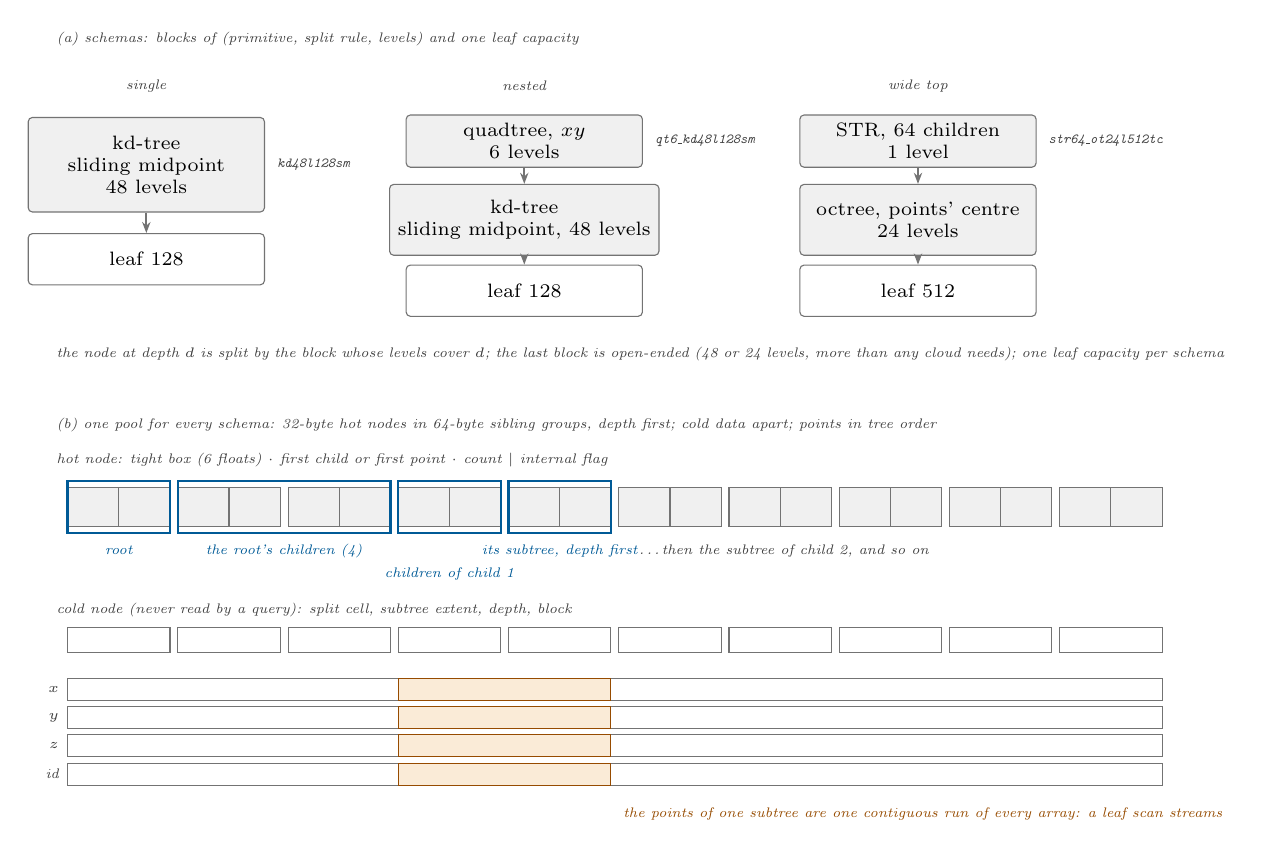
\begin{tikzpicture}[x=1mm, y=1mm, font=\scriptsize]
  % ------------------------------------------------------------ left: three schemas
  \node[mdslabel, anchor=west] at (-2, 22) {(a) schemas: blocks of (primitive, split rule, levels) and one leaf capacity};
  % single
  \node[mdslabel] at (10, 16) {single};
  \node[mdsbox, minimum width=30mm, minimum height=12mm] (s1) at (10, 6) {kd-tree\\sliding midpoint\\48 levels};
  \node[mdsbox, minimum width=30mm, fill=white] (sl) at (10, -6) {leaf 128};
  \draw[mdsflow] (s1) -- (sl);
  \node[mdslabel, anchor=west] at (26, 6) {\schema{kd48l128sm}};
  % nested
  \node[mdslabel] at (58, 16) {nested};
  \node[mdsbox, minimum width=30mm] (n1) at (58, 9) {quadtree, $xy$\\6 levels};
  \node[mdsbox, minimum width=30mm, minimum height=9mm] (n2) at (58, -1) {kd-tree\\sliding midpoint, 48 levels};
  \node[mdsbox, minimum width=30mm, fill=white] (nl) at (58, -10) {leaf 128};
  \draw[mdsflow] (n1) -- (n2);
  \draw[mdsflow] (n2) -- (nl);
  \node[mdslabel, anchor=west] at (74, 9) {\schema{qt6\_kd48l128sm}};
  % wide top
  \node[mdslabel] at (108, 16) {wide top};
  \node[mdsbox, minimum width=30mm] (w1) at (108, 9) {STR, 64 children\\1 level};
  \node[mdsbox, minimum width=30mm, minimum height=9mm] (w2) at (108, -1) {octree, points' centre\\24 levels};
  \node[mdsbox, minimum width=30mm, fill=white] (wl) at (108, -10) {leaf 512};
  \draw[mdsflow] (w1) -- (w2);
  \draw[mdsflow] (w2) -- (wl);
  \node[mdslabel, anchor=west] at (124, 9) {\schema{str64\_ot24l512tc}};
  \node[mdslabel, anchor=west, text width=150mm] at (-2, -18)
    {the node at depth $d$ is split by the block whose levels cover $d$; the last block is open-ended (48 or 24 levels, more than any cloud needs); one leaf capacity per schema};

  % ------------------------------------------------------------ right: the pool
  \begin{scope}[shift={(0, -40)}]
    \node[mdslabel, anchor=west] at (-2, 13) {(b) one pool for every schema: 32-byte hot nodes in 64-byte sibling groups, depth first; cold data apart; points in tree order};
    \node[mdslabel, anchor=west] at (-2, 8.5) {hot node: tight box (6 floats) $\cdot$ first child or first point $\cdot$ count $|$ internal flag};
    % hot node lines
    \foreach \i in {0,...,9} {
      \draw[mdsline, fill=mdsfill] (\i*14, 0) rectangle ++(13, 5);
      \draw[mdsline] (\i*14+6.5, 0) -- ++(0, 5);
    }
    % root group (slot 0 pads, slot 1 root) and three sibling groups
    \draw[mdsaccent, thick] (0, -0.8) rectangle ++(13, 6.6);
    \node[mdslabel, text=mdsaccent] at (6.5, -3) {root};
    \draw[mdsaccent, thick] (14, -0.8) rectangle ++(27, 6.6);
    \node[mdslabel, text=mdsaccent] at (27.5, -3) {the root's children (4)};
    \draw[mdsaccent, thick] (42, -0.8) rectangle ++(13, 6.6);
    \node[mdslabel, text=mdsaccent] at (48.5, -6) {children of child 1};
    \draw[mdsaccent, thick] (56, -0.8) rectangle ++(13, 6.6);
    \node[mdslabel, text=mdsaccent] at (62.5, -3) {its subtree, depth first};
    \node[mdslabel, anchor=west] at (72, -3) {\ldots then the subtree of child 2, and so on};
    % cold array
    \node[mdslabel, anchor=west] at (-2, -10.5) {cold node (never read by a query): split cell, subtree extent, depth, block};
    \foreach \i in {0,...,9} {
      \draw[mdsline, fill=white] (\i*14, -16) rectangle ++(13, 3.2);
    }
    % point arrays
    \foreach \j/\lab in {0/$x$, 1/$y$, 2/$z$, 3/id} {
      \draw[mdsline, fill=white] (0, -22-\j*3.6) rectangle ++(139, 2.8);
      \node[mdslabel, anchor=east] at (-0.5, -20.6-\j*3.6) {\lab};
      \draw[mdsout, fill=mdsoutfill] (42, -22-\j*3.6) rectangle ++(27, 2.8);
    }
    \node[mdslabel, anchor=west, text=mdsout] at (70, -36.5) {the points of one subtree are one contiguous run of every array: a leaf scan streams};
  \end{scope}
\end{tikzpicture}%
}
\caption{(a) The schema grammar. A schema is a sequence of blocks, each a primitive with a split rule and a number of levels, and one leaf capacity; a single structure is a schema with one block. (b) Every schema compiles into the same pool: 32-byte hot nodes holding the tight box and the child or point range, two per cache line, children contiguous as a sibling group that starts on a line boundary, subtrees laid out depth first; the data a query never reads lives in a parallel cold array; the points are reordered into tree order as separate coordinate arrays, so every subtree is a contiguous run. Composition changes the split rule at some depths and nothing else.}
\label{fig:grammar}
\end{figure*}


Table~\ref{tab:designspace} lists what an index variant may change. Most of it is familiar: the primitive, its split rule, the leaf capacity and the depth. One option needs a short explanation, because hybrid indexes have been proposed for point clouds several times~\cite{wang2021hybridpointcloud,park2021nestedoctree,ogayar2023nestedlidar}: \emph{nesting}, the composition of several primitives in one hierarchy.

\begin{table}[t]
\centering\footnotesize
\caption{What an index variant may select. A variant is one primitive or a sequence of primitives (nesting), one leaf capacity, a node order and, when out of core, a placement and a cache size.}
\label{tab:designspace}
\begin{tabular}{p{0.24\linewidth}p{0.68\linewidth}}
\toprule
Choice & Options \\
\midrule
Primitive & kd-tree; quadtree; octree; regular grid ($3^3$ cells); hierarchical grid ($4^3$ cells); sort-tile-recursive tree (8, 27 or 64 children) \\
Split rule & kd-tree: median of the longest axis, sliding midpoint, cell centre; quadtree and octree: cell centre or centre of the points' box \\
Leaf capacity & 16 to 32\,768 points \\
Depth & a level count per primitive; the last primitive is open-ended (deep enough for any cloud here) \\
Nesting & a sequence of primitives, each over a number of levels (e.g.\ a 6-level quadtree over a kd-tree) \\
Node order & depth-first or page-blocked \\
Placement & in memory; leaves on a device; hierarchy and leaves on a device; LRU cache size \\
Memory pages & 4\,KiB or 2\,MB (huge pages); child prefetch on or off \\
\bottomrule
\end{tabular}
\end{table}

A nested variant is a sequence of blocks, each a primitive with a split rule and a number of levels, sharing one leaf capacity: the node at depth $d$ is split by the block whose levels cover $d$ (Fig.~\ref{fig:grammar}a). A single structure is the one-block case. In this engine a nested variant is not a different storage scheme: it has the same hot nodes, the same sibling groups, the same leaf arrays and the same traversal as a single structure, and the only thing a second block changes is the split rule, hence the fan-out, at some depths. Two conventions keep the comparison with single structures fair: every variant has one leaf capacity, so a nested variant cannot win by giving its last block a different leaf; and the last block is open-ended, so depth never ends a tree before its leaf capacity does. Without the second convention, nested variants appeared to win on dense scans in our own earlier experiments, by lending a capped kd-tree the levels it was denied; Section~\ref{sec:composition} reports composition under the fair conventions.

\subsection{The search as a source of the best structure}\label{sec:search}

For each cloud and workload, a search on one half of the query trace finds the fastest single structure and the fastest nested variant under the same budget; the other half is held out for every number in this paper. It combines a fixed grid of 55 tuned single structures (every primitive and split rule at leaf capacities from 32 to 32\,768) with a genetic search over one to three blocks, and confirms its finalists by re-timing them in three processes with rotated order. A nested variant is selected only if it is at least 3\% faster than the best single in the median over processes and faster in every process. The search is an instrument here, not a contribution: Section~\ref{sec:rule} shows that a one-feature rule picks nearly as well.

\paragraph{What the engine does not do.} Indexes are static; a changed cloud is rebuilt. Coordinates are single-precision floats in a frame local to the cloud. Reads from the device are synchronous at queue depth one, without prefetching or batching. Points and nodes are not compressed.

\section{Experimental setup}\label{sec:setup}

\subsection{Scenes and cells}\label{sec:scenes}

The study uses \nScenes{} scenes (Table~\ref{tab:scenes}) from three acquisition groups: \emph{ground} scans, terrestrial and mobile laser scans of streets and heritage sites, which are three-dimensional and dense near the scanner; \emph{aerial} surveys of terrain and cities from aircraft and drones, which are 2.5-dimensional; and \emph{forest} scans, where vegetation fills the volume, together with a vegetated urban park. One photogrammetric object scan is used at one million points only. The scenes come from public benchmarks (Semantic3D, Paris-Lille-3D, Toronto-3D), national mapping agencies (PNOA in Spain, LINZ in New Zealand) and surveys of the authors' institution; Table~\ref{tab:scenes} gives the sources and the native point counts.

\begin{table*}[t]
\centering\footnotesize
\caption{The scenes. Flatness is the score of Section~\ref{sec:rule} (a range where it varies with size); cells counts the sizes at which a scene appears, from one million to one billion points. Every cell is a seeded strict subset of the scene's native points, so no cell contains interpolated points.}
\label{tab:scenes}
% generated by scripts/paper/tables.py; do not edit
\begin{tabular}{llllrrl}
\toprule
Scene & Group & Acquisition & Source & Native points & Flatness & Cells \\
\midrule
Alhambra & ground & TLS & own survey, Granada & 99\,999\,776 & 0.28 & 5 (1M--100M) \\
Cathedral & ground & TLS & Semantic3D & 95\,309\,849 & 0.45--0.51 & 4 (1M--50M) \\
DomFountain & ground & TLS & Semantic3D & 121\,466\,218 & 0.41--0.59 & 5 (1M--100M) \\
Lille & ground & MLS, Velodyne HDL-32E & Paris-Lille-3D & 120\,000\,000 & 0.48 & 4 (1M--100M) \\
Neugasse & ground & TLS & Semantic3D & 50\,122\,464 & 0.53 & 3 (1M--25M) \\
OttobrunnCampus & ground & TLS & -- & 111\,782\,240 & 0.56 & 4 (1M--100M) \\
ParisLux & ground & MLS, Velodyne HDL-32E & Paris-Lille-3D & 50\,000\,000 & 0.47 & 3 (1M--25M) \\
Toronto & ground & MLS, 32-line & Toronto-3D & 78\,320\,210 & 0.48 & 3 (1M--25M) \\
\midrule
Aneto & aerial & ALS & PNOA-LiDAR 2023 & 79\,717\,975 & 0.61 & 4 (1M--50M) \\
Barcelona & aerial & ALS & PNOA-LiDAR 2021 & 49\,267\,228 & 0.69 & 3 (1M--25M) \\
SanAndreas & aerial & UAV (senseFly eBee) & -- & 1\,191\,514\,616 & 0.53 & 7 (1M--1B) \\
SolarPlantation & aerial & UAV & own survey, solar plant & 728\,841\,014 & 0.81 & 4 (1M--100M) \\
Waikato Hamilton & aerial & ALS & LINZ Waikato LiDAR & 6\,015\,584\,388 & 0.64 & 7 (1M--1B) \\
\midrule
GaliciaForest & forest & TLS & 22 TLS plots, Galicia & 2\,052\,645\,430 & 0.50 & 8 (1M--1B) \\
GaliciaForest ES 05 & forest & TLS & one GaliciaForest plot & 114\,290\,378 & 0.52 & 5 (1M--100M) \\
Retiro & forest & ALS & PNOA-LiDAR 2024 & 39\,563\,361 & 0.89 & 3 (1M--25M) \\
\midrule
Museum & other & photogrammetry & Sketchfab & 2\,449\,789 & 0.25 & 1 (1M) \\
\bottomrule
\end{tabular}

\end{table*}

A \emph{cell} is one scene at one size. Sizes form a ladder from one million to one billion points, every tier a seeded strict subset of the one above, so that a scaling curve measures size alone and not a changing scene. The \nCells{} cells of the study (Table~\ref{tab:budgets}) are the \nSearchedCells{} that were searched, from one million to 250 million points, and \nTransferCells{} transfer cells at 500 million and one billion points, which reuse the schema selected on the same scene at 250 million and are measured like the rest. Cells up to 50 million points were measured on the workstation and cells of 100 million points and more on the server (Section~\ref{sec:hardware}); no ratio in this paper crosses the two machines.

\begin{table}[t]
\centering\footnotesize
\caption{Cells and budgets per size: the queries replayed from the held-out trace, and for the searched cells the genetic arm's generated schemas per generation, generations and population. The tuned-singles arm is the same 55 schemas at every size.}
\label{tab:budgets}
% generated by scripts/paper/tables.py; do not edit
\begin{tabular}{lrrll}
\toprule
Points & Cells & Queries & Arm & GA budget \\
\midrule
1M & 17 & 3000 & search & 24 $\times$ 2 $\times$ 16 \\
5M & 16 & 3000 & search & 24 $\times$ 2 $\times$ 16 \\
25M & 16 & 2000 & search & 24 $\times$ 2 $\times$ 12 \\
50M & 6 & 1500 & search & 32 $\times$ 3 $\times$ 20 \\
100M & 9 & 1000 & search & 32 $\times$ 3 $\times$ 20 \\
250M & 3 & 600 & transfer & -- \\
500M & 3 & 400 & transfer & -- \\
1B & 3 & 300 & transfer & -- \\
\bottomrule
\end{tabular}

\end{table}

\subsection{Query workloads}\label{sec:workloads}

The queries are the ones a point-cloud processing pipeline issues, not random points. For every cell, three stages of a standard pipeline were run over the cloud and their queries recorded: normal estimation, a $k$-nearest-neighbour query with $k = 16$ at every point; radius outlier removal, a radius query at every point with a radius of four times the cloud's mean point spacing; and Euclidean clustering, a radius query at 2.5 times the spacing. The mean spacing is computed exactly from the nearest-neighbour distances up to 130 million points and from point-anchored blocks above that. Each stage is subsampled uniformly to 20\,000 query centres, so a cell's trace holds 60\,000 queries, one third of them $k$-nearest-neighbour and two thirds radius, in the stage-major order the pipeline produced them.

Each trace is split in half, stratified by query type and parameter with a fixed seed and keeping the original order within each half. The \emph{opt} half is what the search sees and the \emph{test} half is what every number in this paper is measured on. A measurement replays the test half with a uniform stride down to the cell's query budget (Table~\ref{tab:budgets}), so the replayed queries stay spread over the whole cloud and consecutive queries are close in space, as they are in the pipeline. Query centres are stored in world coordinates and transformed to the cloud's local frame in double precision at load time.

Section~\ref{sec:composition} also reports seven variants of this workload with larger radii, larger $k$, and axis-aligned range and count queries built on the same centres, and Section~\ref{sec:ooc} adds a workload of 30 large boxes per cloud for the out-of-core regimes.

\subsection{Measurement protocol}\label{sec:protocol}

Every process is pinned to one core and, on the server, to the memory of that core's socket. Building is timed separately and excluded from every query latency. A schema is warmed up by one untimed pass over the replayed queries before its timed passes, and the timed passes run with telemetry compiled out. A schema's latency is the mean per-query time of a pass; a cell's result for a schema is the median of that mean over three processes that run the schemas in rotated order, so that a slow stretch of the machine hits every schema in turn. Two schemas within 3\% of each other are reported as a tie.

Two timing protocols are used, and the paper says which one each table rests on. In the \emph{interleaved} protocol all indexes of a process are built first and each pass runs one sweep per schema, starting one schema later each pass; this is the protocol of the search and of the held-out e9 numbers, and it is fair between the schemas of one process because they share the same conditions. It is, however, slower than timing a schema alone: with several large indexes resident, a memory-bound tree runs up to about a fifth slower, and Section~\ref{sec:mechanism} shows that most of that penalty is the reach of the translation look-aside buffer, since it nearly disappears on two-megabyte pages. In the \emph{sequential} protocol a schema is built, warmed up and timed before the next is built, which is within a few percent of timing it alone. The comparison with external libraries (Section~\ref{sec:libraries}), whose drivers time one setting after another, and the headline panel at 100 million points (Section~\ref{sec:levers}) use the sequential protocol; ratios are never taken across protocols.

Every pass recomputes the per-query counts and an order-independent hash of the returned identifiers and compares them with the first pass; the same hash is computed by the external drivers, so a library's answers are checked against the engine's query by query. The checks are reported with the results.

\subsection{External libraries}\label{sec:drivers}

Five libraries are timed on the same clouds and traces through one driver protocol: nanoflann~\cite{blanco2014nanoflann} (a sliding-midpoint kd-tree, leaf 10 by default, 16 to 256 swept), the Point Cloud Library~\cite{rusu2011pcl} (its FLANN kd-tree~\cite{muja2009flann}, and its octree search at voxel sizes from the extent over 128 to over 4096), Open3D~\cite{zhou2018open3d} (a FLANN kd-tree over a double-precision matrix), the octree of Behley et al.~\cite{behley2015octree} (bucket 32 by default, 8 to 512 swept; radius queries only), and the R-tree of Boost.Geometry with sort-tile-recursive bulk loading (16 entries per node as documented, 8 to 64 swept). Each driver reads the same cloud in the same local single-precision frame, replays the same stride of the same trace, times each search call alone around the library's own function, warms up with one pass and times ten, and runs in three rounds with the process order rotated. The reported latency is the median over rounds.

\subsection{Hardware}\label{sec:hardware}

The server has two Intel Xeon Gold 6140 processors (18 cores and 24.75\,MB of last-level cache per socket) and 251\,GB of memory, runs Linux with transparent huge pages in \emph{madvise} mode, and compiles the engine with GCC~12; it also holds an NVIDIA Quadro RTX 6000 used for the GPU measurements of Section~\ref{sec:composition}. The workstation has an Intel Core i7-14700KF (a hybrid processor; runs are pinned to a performance core) and 64\,GB of memory, runs Windows~11 and compiles the engine with MSVC. Cells up to 50 million points ran on the workstation and cells of 100 million points and more, the external libraries, the out-of-core and the layout experiments on the server. The server was shared with other users' jobs on other cores throughout; the rotated processes and medians of Section~\ref{sec:protocol} are there to absorb that.

\section{Results}\label{sec:results}
\subsection{Primitive and leaf}\label{sec:levers}

Figure~\ref{fig:levers} and Table~\ref{tab:levers} split, cloud by cloud, the gap between a library default and the fastest structure the search finds into two steps. Three variants are compared on the held-out half of every cloud: the engine's octree default (16 levels, leaf 32); the \emph{best primitive}, the fastest of the engine's nine primitives at their default parameters (leaf 32, default split rule); and the \emph{tuned} structure, the fastest single structure of any leaf, depth and split rule. Every ratio is between variants measured on the same cloud under the same protocol.

\begin{figure}[tb]
\centering
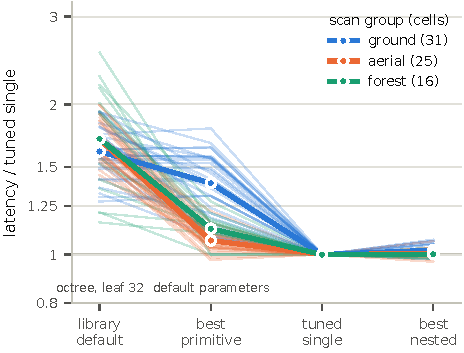
\includegraphics[width=\linewidth]{figures/fig_levers}
\caption{From library default to tuned structure. For each of the \nCells{} held-out clouds, the latency of the octree default and of the best primitive at default parameters, relative to the tuned structure (thin lines); the thick lines are geometric means per scan group.}
\label{fig:levers}
\end{figure}

\begin{table*}[t]
\centering\footnotesize
\caption{The two steps from a default to the tuned structure, on the held-out half: geometric means of per-cloud latency ratios (above 1: the second variant is faster). \emph{Default}: the engine's octree or median-split kd-tree at leaf 32; \emph{best primitive}: the fastest of the nine primitives at default parameters; \emph{tuned}: the fastest single structure of any leaf, depth and split rule. Clouds up to 50M points were measured on the workstation and from 100M on the server, interleaved protocol; no ratio crosses machines.}
\label{tab:levers}
% generated by scripts/paper/tables.py; do not edit
\begin{tabular}{lrrrrrr}
\toprule
Size or group & clouds & \begin{tabular}[b]{@{}c@{}}octree default\\/ best primitive\end{tabular} & \begin{tabular}[b]{@{}c@{}}kd-tree default\\/ best primitive\end{tabular} & \begin{tabular}[b]{@{}c@{}}best primitive\\/ tuned\end{tabular} & \begin{tabular}[b]{@{}c@{}}octree default\\/ tuned\end{tabular} & \begin{tabular}[b]{@{}c@{}}kd-tree default\\/ tuned\end{tabular} \\
\midrule
1M & 17 & 1.477 & 1.167 & 1.174 & 1.770 & 1.380 \\
5M & 16 & 1.344 & 1.336 & 1.256 & 1.745 & 1.699 \\
25M & 16 & 1.256 & 1.244 & 1.293 & 1.610 & 1.612 \\
50M & 6 & 1.207 & 1.114 & 1.241 & 1.465 & 1.387 \\
100M & 9 & 1.303 & 1.268 & 1.193 & 1.568 & 1.527 \\
250M & 3 & 1.630 & 1.441 & 1.055 & 1.718 & 1.542 \\
500M & 3 & 1.547 & 1.399 & 1.036 & 1.612 & 1.499 \\
1B & 3 & 1.455 & 1.365 & 1.089 & 1.560 & 1.527 \\
\midrule
ground & 31 & 1.175 & 1.124 & 1.391 & 1.610 & 1.550 \\
aerial & 25 & 1.533 & 1.571 & 1.067 & 1.703 & 1.730 \\
forest & 16 & 1.504 & 1.103 & 1.127 & 1.707 & 1.255 \\
\midrule
all & 73 & 1.360 & 1.255 & 1.210 & 1.659 & 1.532 \\
\bottomrule
\end{tabular}

\end{table*}

Over all \nCells{} clouds the octree default is \leverOctreeDefaultTuned$\times$ slower than the tuned structure and the median-split kd-tree default \leverKdDefaultTuned$\times$. Choosing the primitive closes a factor of \leverOctreeDefaultPrimitive{} from the octree and \leverKdDefaultPrimitive{} from the kd-tree; tuning the leaf capacity, the depth and the split rule of that primitive closes a further \leverPrimitiveTuned$\times$.

The two steps trade places between scan groups, which is why one default cannot serve all of them. On the aerial surveys the primitive is the lever: a quadtree beats the octree and kd-tree defaults by half again, because a 2.5-dimensional scene gains nothing from splitting height, and once the quadtree is chosen little is left to tune. On the ground scans the primitive step is small, since a kd-tree at leaf 32 is already close to the octree, and the tuning step is large: these scans want the sliding-midpoint split, deep trees and leaves of 64 to 128 points, none of which a default provides. The forest scans sit between. In every group the two steps together give a factor between 1.5 and 1.8.

The decomposition holds at every size. The default gap does not grow with the cloud: it is as large at one million points as at one billion, so what the defaults miss is not scale but the fit of the primitive and the leaf to the scene. The 250M, 500M and 1B clouds reuse the structure selected at 250M on the same scene and lose nothing by it, so a structure chosen on a quarter of the points transfers to the whole cloud.

\paragraph{The headline panel at 100M, timed sequentially.} The ratios above come from the interleaved protocol, which slows memory-bound trees by up to a fifth (Section~\ref{sec:protocol}). Table~\ref{tab:panel} therefore re-times the nine 100M clouds sequentially, on both page sizes: the two defaults, the flatness rule's pick (Section~\ref{sec:rule}) and the searched best. The picture holds. The octree default is \panelOctreeDefaultBase$\times$ the searched best and the kd-tree default \panelKdDefaultBase$\times$; the rule's pick is \panelRuleBase$\times$, within a few percent on every cloud; and the searched best is \panelPickOracleBase$\times$ the fastest structure of the panel. On 2\,MB pages every ratio moves by a point or two in the same direction, because the variants with more and smaller leaves gain more (Section~\ref{sec:ram}).

\begin{table*}[t]
\centering\footnotesize
\caption{The headline panel at 100 million points, sequential protocol, geometric mean (range, clouds) of per-cloud ratios, on 4\,KiB and on 2\,MB pages. \emph{Searched best}: the structure selected by the search on the other half of the trace; \emph{flatness rule}: the pick of the rule of Section~\ref{sec:rule}. The last row is each structure on 2\,MB pages over itself on 4\,KiB pages.}
\label{tab:panel}
% generated by scripts/paper/tables.py; do not edit
\begin{tabular}{lrr}
\toprule
Ratio & base: 4 KiB pages & huge pages \\
\midrule
octree default / pick & 1.723 (1.31--2.20, $n$=9) & 1.755 (1.32--2.24, $n$=9) \\
kd default / pick & 1.464 (1.14--2.36, $n$=9) & 1.511 (1.15--2.52, $n$=9) \\
rule / pick & 1.009 (1.00--1.04, $n$=9) & 1.041 (1.01--1.08, $n$=9) \\
pick / best single & 1.002 (1.00--1.01, $n$=9) & 1.000 (1.00--1.00, $n$=9) \\
nested / best single & 1.021 (1.00--1.05, $n$=9) & 1.032 (0.99--1.11, $n$=9) \\
stage B winner / pick & 2.425 (2.17--2.79, $n$=3) & 2.514 (2.28--2.84, $n$=3) \\
\midrule
huge / base, single schemas &  & 0.958 (0.92--1.01, $n$=45) \\
huge / base, nested schemas &  & 0.957 (0.92--0.99, $n$=12) \\
\bottomrule
\end{tabular}

\end{table*}

\subsection{A one-feature rule}\label{sec:rule}

If the gain is in the primitive and its leaf, the practical question is whether every cloud needs its own search or whether a fixed rule captures the gain. Table~\ref{tab:rule} answers it on the \nRuleCells{} searched clouds. The reference is the \emph{per-cloud best}, the fastest single structure found on each cloud's search half; a rule's \emph{regret} is the latency of the structure it picks over that best. Every rule picks from the 55 tuned structures and is fitted leave-one-scene-out: when a cloud is scored, every cloud of the same scene at every size is left out of the fit, so a rule never sees the cloud it is judged on. Two latency columns are reported, the instrumented pass and the mean of the timed passes, because the two rank close variants differently and a rule should not depend on which one is read.

\begin{table*}[t]
\centering\footnotesize
\caption{Fixed rules against the per-cloud best (the fastest single structure on the search half), \nRuleCells{} searched clouds, fitted leave-one-scene-out. Regret is the geometric mean of the rule's latency over the best's; p90 its 90th percentile; the last column counts clouds where the rule is more than 15\% off. Left: the instrumented pass; right: the timed passes.}
\label{tab:rule}
% generated by scripts/paper/tables.py; do not edit
\begin{tabular}{lrrrrrr}
\toprule
Rule & regret & p90 & cells $>1.15$ & regret & p90 & cells $>1.15$ \\
\midrule
library octree default, leaf 32 & 1.746 & 2.18 & 68 & 1.950 & 2.77 & 68 \\
library kd-tree default, leaf 32 & 1.630 & 1.98 & 67 & 1.619 & 2.05 & 68 \\
floor: best of the 55 tuned singles per cell & 1.011 & 1.05 & 0 & 1.010 & 1.04 & 0 \\
one global schema & 1.067 & 1.21 & 10 & 1.074 & 1.18 & 12 \\
one schema per scan group & 1.078 & 1.23 & 12 & 1.106 & 1.33 & 14 \\
one split on the flatness score & 1.043 & 1.10 & 2 & 1.076 & 1.20 & 12 \\
\bottomrule
\end{tabular}

\end{table*}

\begin{figure}[tb]
\centering
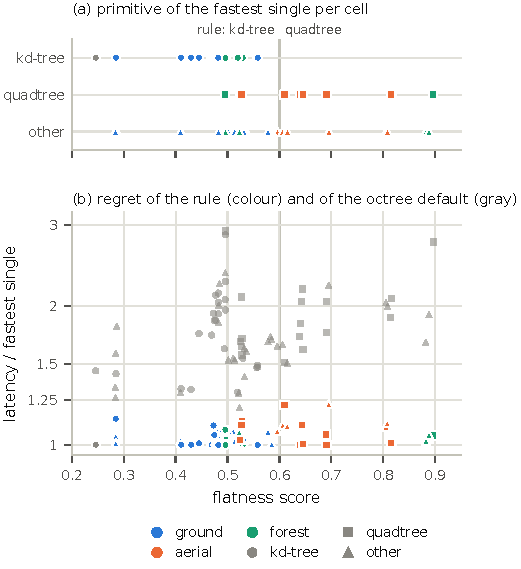
\includegraphics[width=\linewidth]{figures/fig_rule}
\caption{(a) The primitive of each cloud's fastest structure on the search half against the cloud's flatness score; the vertical line is the rule's split. (b) The regret of the one-split rule (coloured by scan group) and of the octree default (gray) per cloud. Marker shape: the primitive of the fastest structure.}
\label{fig:rule}
\end{figure}

The library defaults are the floor of the comparison: the octree default is \octreeDefaultRegret$\times$ the per-cloud best in the instrumented column and \octreeDefaultRegretTimed$\times$ in the timed one, the median kd-tree default \kdDefaultRegret$\times$, and every cloud but one is more than 15\% off. The ceiling is the best of the 55 tuned structures per cloud, at \floorRegret: the grid is dense enough that a search over it loses almost nothing to the open-ended genetic search. One global structure, the same for every cloud, is \globalSchemaRegret$\times$ the per-cloud best: a 48-level sliding-midpoint kd-tree with a leaf of 64 or 128 points, which is already most of the way. One structure per scan group does worse (\groupSchemaRegret), because the forest group mixes a flat park, where a quadtree wins, with a volumetric forest, where a kd-tree does.

The rule that works is a single split on one feature. A regression tree of depth one over thirteen cloud features (point count, density, aspect ratios, height statistics, covariance shape, occupancy, verticality and flatness) chooses the \emph{flatness score} in every fold, with the same threshold in both latency columns:
\[
\text{flatness} = \bigl(1 - \tfrac{\text{z extent}}{\max(\text{x extent}, \text{y extent})}\bigr)\cdot\tfrac{\text{planarity} + 1 - \text{scattering}}{2},
\]
from the extents of the cloud and the covariance eigenvalues of a fixed-seed sample of its points. Below 0.60 the rule picks the sliding-midpoint kd-tree with 48 levels and leaf 128; above it, a quadtree with 16 levels and a leaf of 64 to 128. Its regret is \ruleRegret{} in the instrumented column and \ruleRegretTimed{} in the timed one, with a 90th percentile of \ruleRegretP{} and \ruleCellsOver{} clouds more than 15\% off. In log terms the rule closes \ruleCapturePct\% of the distance from the octree default to the per-cloud best; what the search adds on top, four to eight percent, is about the measurement noise of the per-cloud best itself, which is the minimum over some 120 noisy candidates whose repeat coefficient of variation is several percent. A tree of depth two fits no better and picks a different second feature in each fold: with sixteen scenes there is nothing more to learn.

Figure~\ref{fig:rule}a shows why one feature suffices. The score separates the 2.5-dimensional scenes, the aerial terrain and cities and the park, where the fastest structure is a quadtree, from the three-dimensional ones, the ground scans and the forests, where it is a kd-tree. The one scene the rule misplaces is a UAV terrain survey whose score of 0.53 falls on the kd-tree side, and that scene is most of the aerial regret in Figure~\ref{fig:rule}b. On every other cloud the rule is within a few percent of the per-cloud best, where the octree default is between 1.3 and 3 times off.

Two caveats bound the claim. The rule was fitted and scored on the search half; on the clouds where its pick, or a structure with the same primitive, leaf and depth, happened to be among the finalists timed on the held-out half, it is within a fraction of a percent of the best timed structure there, but that sample is biased towards clouds where the rule's pick was already a finalist. And the leaf capacities it names were measured on 4\,KiB pages; Section~\ref{sec:ram} shows that the optimum moves on a machine with transparent huge pages enabled.

\FloatBarrier
\subsection{Against the libraries}\label{sec:libraries}

A gap between a library default and a tuned structure measured inside one engine could be a property of that engine. Table~\ref{tab:libraries} times five libraries on \nLibraryCells{} cells (one scene at 1M, five at 25M, nine at 100M) under the sequential protocol of Section~\ref{sec:protocol}, each at its default and across its main parameter, next to our own defaults and the rule's pick, all relative to the cell's selected schema. Every library's answers were checked against the engine's query by query: no count differs anywhere, and the identifier sets differ only on $k$-nearest-neighbour queries whose $k$-th and $(k{+}1)$-th neighbours lie at the same single-precision distance, which the libraries break differently.

\begin{figure*}[tb]
\centering
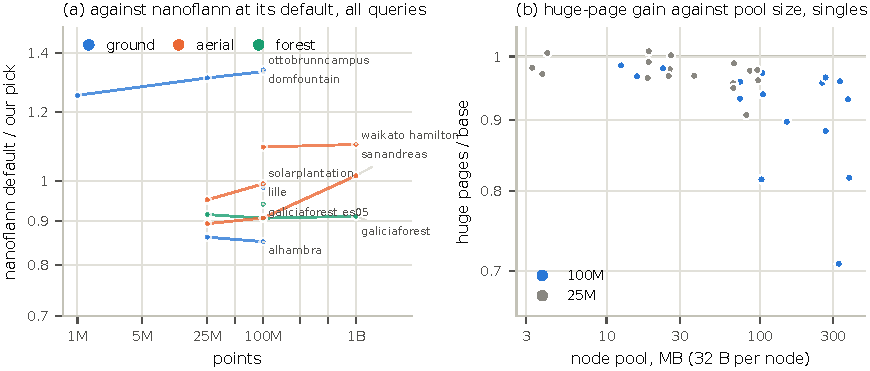
\includegraphics[width=\textwidth]{figures/fig_scale}
\caption{(a) nanoflann at its default leaf over the cell's selected schema, per scene and size, all queries of the trace, sequential protocol. (b) The huge-page arm over the base arm for every single structure of Section~\ref{sec:mechanism} against its node pool size: the gain grows with the pool, and the largest pools gain most.}
\label{fig:scale}
\end{figure*}

\begin{table}[t]
\centering\footnotesize
\caption{External libraries on the held-out traces, latency per query relative to the cell's selected schema (above 1: slower than our pick), geometric means over \nLibraryCells{} cells, for the trace's query mix and for its radius and $k$-nearest-neighbour queries separately; the last column is each library's own default over its best setting. Sequential protocol, median of three rotated rounds.}
\label{tab:libraries}
% generated by scripts/paper/tables.py; do not edit
\begin{tabular}{lrrrr}
\toprule
Library, setting & all & radius & kNN & own lever \\
\midrule
ours, octree default & 1.73 & 1.91 & 1.52 &  \\
ours, kd-tree default & 1.42 & 1.57 & 1.24 &  \\
ours, rule pick & 1.01 & 0.96 & 1.06 &  \\
nanoflann kd, def. & 1.02 & 1.27 & 0.72 & 1.07 \\
nanoflann kd, best & 0.95 & 1.18 & 0.68 &  \\
PCL KdTreeFLANN, def. & 2.59 & 3.51 & 1.58 &  \\
Open3D KDTreeFlann, def. & 1.60 & 2.13 & 1.00 &  \\
unibn octree, def. & -- & 1.65 & -- & 1.05 \\
unibn octree, best & -- & 1.56 & -- &  \\
Boost R-tree, def. & 2.46 & 2.32 & 2.50 & 1.04 \\
Boost R-tree, best & 2.37 & 2.24 & 2.40 &  \\
\bottomrule
\end{tabular}

\end{table}

\paragraph{nanoflann ties the tuned pick.} At its default leaf of ten points nanoflann~\cite{blanco2014nanoflann} is \nanoflannDefaultAll$\times$ our selected schema over the query mix, and at its best leaf of 16 to 32 it is \nanoflannBestAll$\times$: a tie at the default and a small win when tuned. The tie is made of two opposite differences. nanoflann is faster on every $k$-nearest-neighbour cell (\nanoflannDefaultKnn$\times$ at its default, \nanoflannBestKnn$\times$ at its best), because it updates the distance to a child cell along the split axis incrementally where our traversal recomputes a three-dimensional box distance per child. Our engine is faster on the radius queries of most cells (nanoflann at \nanoflannDefaultRadius$\times$ and \nanoflannBestRadius$\times$), because its leaves stream through reordered coordinate arrays where nanoflann gathers the original points through an index. Leaf for leaf, the two engines are at parity, and nanoflann's default is already the right structure for a three-dimensional scene: a sliding-midpoint kd-tree with a small leaf. Figure~\ref{fig:scale}a shows the ratio per scene and size: flat across the range measured here, with a slight drift in our favour as the cloud grows.

\paragraph{At a billion points.} The three clouds of the study that reach one billion points (a forest and two aerial surveys) were timed against nanoflann under the same sequential protocol, with a thousand replayed queries. The tie holds: nanoflann's default is \anchorNanoflannDefaultAll$\times$ the selected schema over the query mix (\anchorNanoflannDefaultMin{} to \anchorNanoflannDefaultMax{} across the three) and \anchorNanoflannBestAll$\times$ at its best leaf, ahead on the $k$-nearest-neighbour queries (\anchorNanoflannDefaultKnn$\times$) and behind on the radius queries (\anchorNanoflannDefaultRadius$\times$), as at every smaller size; it is ahead on the forest scan and behind on the two aerial ones, where the selected schema is a quadtree. Our own defaults are \anchorOursOctreeDefault{} and \anchorOursKdDefault$\times$ the pick there, the same gap as below. Nothing in the data suggests that either engine pulls away at a billion points.

\paragraph{The other libraries are slower by implementation.} The FLANN kd-tree of the Point Cloud Library is \pclKdAll$\times$ our pick, the Boost.Geometry R-tree \boostAll$\times$, Open3D's kd-tree \openThreeDAll$\times$, and the octree of Behley et al.\ \unibnRadius$\times$ on the radius queries it supports; the Point Cloud Library's octree search is \pclOctreeAll$\times$, and forty times off on the forest scans, where its voxels are either empty or overfull. Each library's own parameter recovers between \libraryLeverMin{} and \libraryLeverMax$\times$, so these gaps are not a matter of tuning: three implementations of the same kd-tree span a factor of 2.6 among themselves, which is the spread Elseberg et al.~\cite{elseberg2012comparison} found a decade ago. The structure a library implements and how it implements it both matter; the composition of structures does not appear in either.

\paragraph{What this does to the default gap.} Our own octree and median kd-tree defaults at leaf 32 are \oursOctreeDefaultOverPick$\times$ and \oursKdDefaultOverPick$\times$ the pick on these cells, and the rule's pick \ruleOverPick$\times$. The 1.6 to 1.7$\times$ gap of Section~\ref{sec:levers} is therefore the gap of a particular pair of defaults, an octree and a median-split kd-tree at a small leaf, and not of library defaults in general: a user of nanoflann already has the right structure for three-dimensional scenes, and a user of PCL or Open3D loses more to the implementation than to the structure. The claim the data supports is narrower and more useful than "defaults leave 1.7$\times$ on the table": choose a sliding-midpoint kd-tree for three-dimensional scenes and a quadtree for 2.5-dimensional ones, give it a leaf of 64 to 128 points, and then the implementation is what is left.

\subsection{Memory layout in RAM}\label{sec:ram}\label{sec:mechanism}

With the index in memory, a query's time is set by where its nodes and points sit in the cache and translation hierarchy, not by how many it touches. This section prices every visit by depth (Figure~\ref{fig:depth}), then changes the layout under a fixed structure: page size, prefetching of child groups, and the leaf capacity on either page size.

\begin{figure*}[tb]
\centering
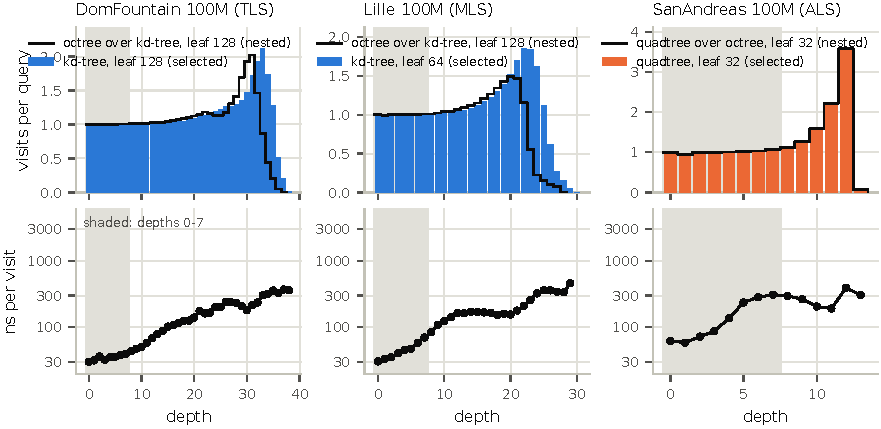
\includegraphics[width=\textwidth]{figures/fig_depth}
\caption{Visits per query (top) and nanoseconds per visit (bottom) by depth for the searched best structure of three 100M clouds, instrumented pass, sequential protocol. The shaded depths are the top eight levels. The nanoseconds of the instrumented pass include the telemetry and sum to about 1.25 times the timed latency; the shares between depths are what the figure is for.}
\label{fig:depth}
\end{figure*}

\paragraph{A visit costs 35\,ns at the top of a tree and 350 at a leaf.} On the DomFountain kd-tree a visit in the top eight levels costs \visitCostTopNs\,ns, one in the middle levels \visitCostMiddleNs\,ns and one in the deepest four \visitCostLeafNs\,ns: an order of magnitude within one tree. The top levels stay in cache for every query of a coherent trace and the deep levels do not. On the ground and mobile scans the top eight levels are \topLevelsShareDomFountain\% of a query's time; on the aerial terrain, where consecutive queries lie far apart, even the top levels miss and the leaves hold half the time.

\paragraph{Node counts do not predict time.} A least-squares model of latency on visited nodes, tested points and returned points, fitted per cloud on the instrumented search-half runs, predicts the gap from the octree default to the per-cloud best at a fraction of its size; adding box tests and tree size as terms does not repair it. One cloud makes the point: on DomFountain at 25M the octree default visits \exampleOctreeVisits{} nodes and tests \exampleOctreePoints{} points per query in \exampleOctreeUs\us, and the fastest structure, a \exampleOracleName, visits \exampleOracleVisits{} nodes and tests \exampleOraclePoints{} points in \exampleOracleUs\us, from a tree of \exampleOracleNodes{} million nodes against \exampleOctreeNodes{} million. More visits, more points, a third of the nodes, and a third less time. In memory no count the engine records ranks structures; only timing does.

\paragraph{Huge pages and prefetching.} Table~\ref{tab:layout} times a panel of structures (the searched best, the rule's picks, the library defaults and two wide structures) on three scenes at 25M and 100M under four variants of the same binary: as it is; with the node pool and point arrays on 2\,MB pages; with the next level prefetched when a child is pushed; and with both. Each ratio compares a structure with itself in the same process group. Huge pages speed up every tree, in proportion to its pool: \hugeSinglesHundredM$\times$ over the 100M structures, \hugeBigPools$\times$ for pools of 64\,MB or more against \hugeSmallPools$\times$ below, \hugeSinglesTwentyFiveM$\times$ at 25M, and down to \hugeMin$\times$ for the largest pool in the panel, a 10-million-node quadtree on SanAndreas (\hugeAloneQt$\times$ when that structure is timed alone). A 75\,MB pool is some 18\,000 pages of 4\,KiB against a second-level translation buffer of 1\,500 entries, so on small pages every cold visit pays a page walk on top of its cache miss, and the 2\,MB page removes it. Prefetching the next level helps the binary and four-way trees, whose pushed child group is one or two cache lines, by up to \prefetchMin$\times$, and hurts the 64-way hierarchical grid by \prefetchHGrid$\times$ on every cloud: its two-kilobyte child group is streamed by the box tests anyway and the prefetches are extra traffic. The two do not add (\bothSinglesHundredM$\times$ together), because they hide the same miss. These ratios were taken interleaved, with several large indexes resident; timed sequentially on the nine 100M clouds of Table~\ref{tab:panel}, huge pages give \panelHugeOverBaseSingles$\times$ (\panelHugeOverBaseSinglesMin{} to \panelHugeOverBaseSinglesMax), with the same ordering by pool size. The interleaved figure includes the translation-buffer pressure that co-resident indexes add; the sequential one is what a lone index gains.

\begin{table*}[t]
\centering\footnotesize
\caption{Layout variants over the unchanged binary, geometric mean (range) of per-structure latency ratios (below 1: the variant is faster), three scenes at 25M and 100M, interleaved in rotated process groups. Pools are the hot-node arrays at 32 bytes per node; the last row is the 64-way hierarchical grid and the variants built on it.}
\label{tab:layout}
% generated by scripts/paper/tables.py; do not edit
\begin{tabular}{lrrr}
\toprule
Structures (count) & huge pages\,/\,base & child prefetch\,/\,base & both\,/\,base \\
\midrule
100M points, all structures (17) & 0.915 (0.71--0.99) & 0.941 (0.72--1.12) & 0.928 (0.69--1.10) \\
100M points, node pool $\geq$ 64 MB (14) & 0.902 (0.71--0.97) & 0.911 (0.72--0.97) & 0.896 (0.69--0.97) \\
100M points, node pool $<$ 64 MB (3) & 0.978 (0.97--0.99) & 1.096 (1.08--1.12) & 1.094 (1.09--1.10) \\
25M points, all structures (17) & 0.974 (0.91--1.01) & 0.970 (0.90--1.10) & 0.970 (0.86--1.11) \\
hierarchical grid, 64-way (8) & 0.982 (0.97--1.01) & 1.092 (1.08--1.12) & 1.093 (1.08--1.11) \\
\bottomrule
\end{tabular}

\end{table*}

\paragraph{The interleaving penalty is translation reach.} The kd-tree timed alone is \aloneOverInterleavedKdBase$\times$ its interleaved time on small pages and \aloneOverInterleavedKdHuge$\times$ on huge pages, while the octree keeps a few percent either way (\aloneOverInterleavedOtBase{} and \aloneOverInterleavedOtHuge). For the memory-bound trees, timing several indexes in one process costs what their pages cost in the translation buffer, which is why every headline ratio of this paper is re-timed sequentially.

\paragraph{The leaf on both page sizes.} Table~\ref{tab:leaflever} sweeps the leaf capacity of the rule's two primitives from 16 to 1\,024 points on the nine 100M clouds, sequentially, on both page sizes. On 4\,KiB pages the kd-tree's best leaf is 64 or 128 on eight of the nine clouds; leaf 32 costs \leafKdOverThirtyTwoBase$\times$ the best and leaf 128 \leafKdOverHundredTwentyEightBase$\times$. On huge pages the best leaf moves down in \leafShiftPairs{} of \leafPairs{} cloud--primitive pairs, all but one of them kd-trees, to 16 or 32 points on five clouds; the small-leaf penalty halves to \leafKdOverThirtyTwoHuge$\times$ and leaf 128 now costs \leafKdOverHundredTwentyEightHuge$\times$. The quadtree wants a larger leaf, 128 to 512 points on the aerial scenes, and its leaf-128 pick stays within \leafQtOverHundredTwentyEightBase$\times$ of the best in either mode, while leaf 32 costs it \leafQtOverThirtyTwoBase$\times$. The worst leaf of the sweep costs \leafWorstMin{} to \leafWorstMax$\times$ the best. The leaf is a lever of the same order as the primitive, its optimum depends on the page size as much as on the structure, and the rule's 64 to 128 is a safe choice on either.

\begin{table*}[t]
\centering\footnotesize
\caption{The leaf capacity on nine 100M clouds, sequential protocol, 4\,KiB and 2\,MB pages: the best leaf per cloud (count of clouds), and the latency at leaf 32, at leaf 128 and at the worst leaf of the sweep over the latency at the best leaf, geometric mean (range).}
\label{tab:leaflever}
% generated by scripts/paper/tables.py; do not edit
\begin{tabular}{llllrr}
\toprule
Primitive & Pages & best leaf (cells) & leaf 32\,/\,best & leaf 128\,/\,best & worst\,/\,best \\
\midrule
kd-tree, sliding midpoint & 4 KiB & 16 (1), 64 (4), 128 (4) & 1.076 (1.02--1.18) & 1.013 (1.00--1.04) & 1.557 (1.40--1.77) \\
 & 2 MB & 16 (3), 32 (2), 64 (1), 128 (3) & 1.040 (1.00--1.14) & 1.036 (1.00--1.10) & 1.576 (1.40--1.83) \\
quadtree, points' centre & 4 KiB & 64 (2), 128 (2), 256 (3), 512 (2) & 1.315 (1.03--1.86) & 1.037 (1.00--1.14) & 1.689 (1.41--2.50) \\
 & 2 MB & 64 (1), 128 (3), 256 (3), 512 (2) & 1.297 (1.03--1.81) & 1.037 (1.00--1.11) & 1.691 (1.41--2.47) \\
\bottomrule
\end{tabular}

\end{table*}

% PENDING (battery 2x, results/eval_traces/threads_makinon2): page-blocked against depth-first node order in RAM,
% single-threaded and at 18/36 threads, both page sizes.

\FloatBarrier
\subsection{Out of core}\label{sec:ooc}

When the points no longer fit in memory, the leaf store of Section~\ref{sec:placement} writes each leaf's points to a file in tree order and reads them back on demand with the operating system's cache bypassed. Three placements result: everything in memory (the control), the leaves on the device with the hierarchy in memory, and both on the device, with the hierarchy read page by page. Each placement can add a least-recently-used cache sized as a fraction of the store. Five 100M clouds, their pipeline traces, the dense segment and a workload of 30 large boxes per cloud were run through every placement on a panel of kd-trees, quadtrees, octrees, hierarchical grids and STR trees with leaves from 128 to 32\,768 points, on the four devices of Table~\ref{tab:devices}.

% PENDING (batteries 2v and 2w, results/eval_traces/devices_{makinon2,workstation}): measured latency per device and
% placement (table + figure), best leaf per device, latency against cache size on the dense segment (figure), and
% page-blocked against depth-first hierarchy reads. The paragraphs below hold the modelled results of the first
% battery and are rewritten on the measured data.

\paragraph{The leaf follows the device.} In memory the best structures have leaves of 32 to 128 points; with the leaves on an SSD they have 512 to 2\,048, on a hard disk 8\,192, and for the large boxes 32\,768. The leaf should cost about as much to scan as a read costs to issue, so it follows the device's latency--bandwidth product. The primitive stays: on every cloud the best structure out of core has the primitive of the in-memory pick, the kd-tree on the ground and forest scans and the quadtree on the aerial ones, and at the device's leaf the rule's primitive is within a few percent of it.

\paragraph{Keep the hierarchy in memory.} A 100M-point hierarchy at the device's leaf is \hierarchyMbMin{} to \hierarchyMbMax\,MB. Keeping it in memory makes the best structure \pagedOverPinnedMinNoCache{} to \pagedOverPinnedMaxNoCache$\times$ faster than the best structure with the hierarchy paged and no cache, and \pagedOverPinnedMinCache{} to \pagedOverPinnedMaxCache$\times$ faster than with a one-percent cache. For comparison, reading the same boxes through a cloud-optimised point cloud reader (COPC) was about 26 times slower than the leaf store's best structure on the same drive, so the store is not a weak baseline.

\paragraph{Caveats.} Reads are synchronous at queue depth one, where a real store would prefetch or batch; the cache is one policy; and the strided trace re-reads almost no leaf, which is why the dense segment is reported alongside it.

\FloatBarrier
\section{Discussion}\label{sec:discussion}

\subsection{Why hybrid indexes have looked good}

Four things made composed hierarchies look faster than they are, and the study met all four before it controlled them.

\paragraph{Untuned baselines.} Every hybrid index we know of was compared against single structures at a library's default parameters, or at a depth cap that the single could not escape. In our own earlier battery, nested schemas won on dense ground scans by up to a quarter, and the whole margin was a depth cap of 22 levels on the sliding-midpoint kd-tree: a quadtree prefix lent the kd-tree tail the levels it was denied. With the cap lifted (Section~\ref{sec:grammar}), the margin was gone in every cell. Against a tuned single, over \nCells{} cells, there is no margin to find.

\paragraph{Node counts.} Hybrids reduce the number of nodes a query enters, and node counts are easy to report. But a visit costs \visitCostTopNs\,ns near the root and \visitCostLeafNs\,ns at a leaf (Section~\ref{sec:mechanism}), and the visits a wide prefix removes are the cheap ones: in cache for every query of a coherent workload. A count of visits is not a cost, and the fitted count models of Section~\ref{sec:mechanism} explain less than half of the lever between a default and a tuned single.

\paragraph{Paged hierarchies.} The nested structures of Ogayar-Anguita et al.~\cite{ogayar2023nestedlidar} were measured in a store where every node load was a file. There, a wide top does spare loads, and Section~\ref{sec:ooc} reproduces the gain in exactly that regime and nowhere else: with the hierarchy paged from a slow device and no cache, a quadtree or grid prefix is adopted in \oocPagedAdopted{} of \oocPagedCells{} cells. The regime is a choice, and an expensive one: pinning the \hierarchyMbMin{} to \hierarchyMbMax\,MB hierarchy of a 100M-point cloud makes any schema \pagedOverPinnedMinNoCache{} to \pagedOverPinnedMaxNoCache$\times$ faster than the best paged one.

\paragraph{Noisy comparisons.} Two schemas timed in different processes, or interleaved with different companions, differ by up to fifteen percent for no reason (the null pair of Section~\ref{sec:mechanism}). A study that reports a nested schema a few percent ahead of a single without rotated processes, medians and an every-process rule has reported the noise. Our adoption rule (Section~\ref{sec:search}) is conservative by design, and the one cell it would have called a win at the 3\% band dissolves under it.

\subsection{What transfers}

The primitive transfers. The flatness score chooses a kd-tree or a quadtree once per scene, and that choice holds from one million to one billion points, from the workstation to the server, and from memory to every out-of-core regime measured: the best single with the leaves on a device has the primitive of the in-memory pick in every cloud. The leaf does not transfer: it follows the device, from 64 to 128 points in memory to 512 or 2\,048 on a solid-state drive and 8\,192 on a hard disk, and it follows the page size, since the huge-page gain is largest for the schemas with the most nodes. A rule for practitioners therefore has two parts, a primitive from the scene's geometry and a leaf from the device's latency--bandwidth product and page size, and neither part is a second primitive.

\subsection{Recommendations}

For a three-dimensional scene (terrestrial or mobile scans, forests, heritage), a sliding-midpoint kd-tree with a leaf of 64 to 128 points, as deep as the data takes it; nanoflann's default is already this structure. For a 2.5-dimensional scene (aerial terrain and cities), a quadtree splitting at the points' centre with a leaf of 64 to 128. Enable transparent huge pages for any index whose node pool exceeds a few tens of megabytes: the gain is \hugeBigPools$\times$ for pools over 64\,MB here, and a server in \emph{always} mode gets it for free. Do not prefetch children of wide nodes. When measuring, pin the process, rotate the order, take medians, and time structures alone or say that they were interleaved. For library authors, the gap between implementations of the same kd-tree is 2.6$\times$ (Section~\ref{sec:libraries}), larger than any structural lever in this paper except the primitive; an octree at leaf 32 is a poor default for dense scans, and an index that reorders its points into tree order wins the radius queries.

\subsection{When composition could still pay}

The study closes the in-memory question for neighbourhood queries on static point clouds and the out-of-core question for hierarchies that fit in memory. It leaves three regimes open. A hierarchy that must be paged from a slow device without a cache, as in a streaming viewer that holds nothing between frames, is where the 2023 result lives, and a page-blocked layout of the pool should be tried before a second primitive. A kernel that is bound by divergence rather than by memory could reward a shallower, wider top; our GPU pass was not, and a specialised GPU kd-tree beat every schema of ours by \oursOverCudaKdTree$\times$, so the implementation is the first thing to fix there. And dynamic settings, where points arrive and leave and the cost is the update rather than the query, were not measured.

\subsection{Threats to validity}

Cells of 100 million points and more, the libraries, the out-of-core and the layout experiments ran on one server, shared with other users on other cores; the smaller cells ran on one workstation; no ratio crosses the machines, but the absolute latencies are those of two processors. The out-of-core devices are modelled from exact read and byte counts with per-class costs, because the drive at hand was not steady; the model has one cache policy and synchronous reads. The query traces are the queries three pipeline stages issue, derived from the cloud's spacing rather than recorded inside a third-party pipeline, and within a scene density co-varies with size, since the tiers are subsets of one scan. The genetic search is one search method; a budget-matched random search matched it in an earlier battery, so the oracle does not depend on it, but the 55-schema grid bounds what any rule can pick. The rule was fitted on sixteen scenes and scored on the opt half. The external libraries were built from conda-forge without AVX for the two whose search code is precompiled, which may overstate their gap by some percent. Finally, two compiler effects would have invalidated the layout battery had they gone unnoticed: the compiler inlined the traversal templates into their entry points and slowed the default path by up to fifteen percent, and it deleted the prefetch arm entirely because a routine that only prefetches has no visible effect; both were caught by an A/B against the previous binary and by reading the disassembly, and the lesson, that a prefetch experiment must be verified in the binary and not in the source, belongs in any paper that reports one.

\section{Conclusions}\label{sec:conclusions}

We set out to measure, in one engine and over \nCells{} cells of \nScenes{} scenes from one million to one billion points, where the query speed of a point-cloud spatial index comes from. The answer has three parts. The primitive and its leaf account for the whole gain between a library default and the best structure a search can find, a factor of \leverOctreeDefaultTuned{} over an octree default and \leverKdDefaultTuned{} over a median kd-tree; a single split on the scene's flatness picks the primitive within \ruleRegret{} to \ruleRegretTimed{} of a per-cloud search, and nanoflann's default already embodies the right choice for three-dimensional scenes. Composing primitives into nested hierarchies adds nothing once the hierarchy is in RAM: \nestedPickedAll{} of \nCells{} cells in memory, none of seven workloads, none on the GPU, none under emulated node costs, and \oocInRamAdopted{} of \oocInRamCells{} out-of-core cells with the leaves on a device. It pays in \oocPagedAdopted{} of \oocPagedCells{} cells with the hierarchy itself paged from a slow device, which is the regime of the result it revisits, and a regime that pinning a few tens of megabytes beats several times over. The mechanism is that a node visit costs an order of magnitude more at a leaf than near the root, so the visits a wide prefix saves are the cheap ones, and node counts do not predict time; the memory layout does, and two-megabyte pages buy more than a second primitive ever did.

The study has limits of its own. It is one engine on two machines; its devices are modelled; its traces come from three pipeline stages; and its rule is fitted on sixteen scenes. What it offers in return is a controlled protocol, a released instrument with its traces, configurations and scripts, and a message that is smaller than the one it replaces and easier to act on: choose the primitive from the geometry, the leaf from the device, the layout from the page size, and measure the rest.


\appendix
\section{Nested variants}\label{sec:composition}

Section~\ref{sec:designspace} describes what a nested variant is in the engine: a sequence of primitives over a range of depths, sharing one leaf capacity, one node pool and one traversal. This appendix reports how such variants fared. The short answer is that they tie the best single structure wherever the hierarchy is in memory, and that they help only when the hierarchy itself is paged from a slow device without a cache, where pinning the hierarchy is several times faster still. Section~\ref{sec:discussion} summarises the result in one paragraph.

\begin{figure*}[tb]
\centering
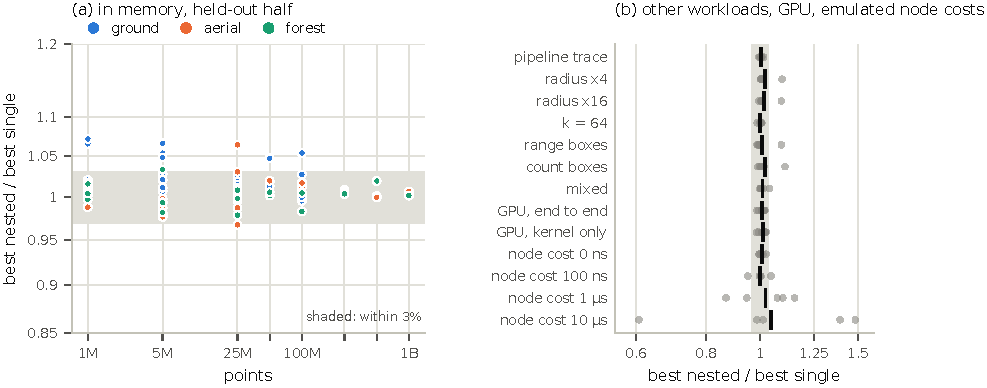
\includegraphics[width=\textwidth]{figures/fig_composition}
\caption{Best nested variant over best single structure. (a) The \nCells{} held-out clouds against their size, coloured by scan group; the band marks the 3\% tie zone. (b) The same ratio on seven workload variants of six 100M clouds, on the GPU for the normal-estimation pass of six clouds at two values of $k$, and under emulated per-node costs of 0 to 10\us{} on five 25M clouds; each dot is one cloud and the bar its geometric mean.}
\label{fig:composition}
\end{figure*}

\begin{table*}[t]
\centering\footnotesize
\caption{Nested variants in memory, held-out half, interleaved protocol: the best nested variant over the best single structure per cloud (geometric mean and range), wins, ties and losses at the 3\% band, the clouds in which the confirmation step adopted a nested variant, and the searched best over the fastest single timed on the held-out half.}
\label{tab:composition}
% generated by scripts/paper/tables.py; do not edit
\begin{tabular}{lrrrrrr}
\toprule
Cells & $n$ & nested picked & nested\,/\,single & range & wins\,/\,ties\,/\,losses & pick\,/\,oracle \\
\midrule
1M & 17 & 0 & 1.015 & 0.99--1.07 & 0\,/\,14\,/\,3 & 1.001 \\
5M & 16 & 0 & 1.013 & 0.98--1.07 & 0\,/\,11\,/\,5 & 1.002 \\
25M & 16 & 0 & 1.006 & 0.97--1.06 & 1\,/\,13\,/\,2 & 1.009 \\
50M & 6 & 0 & 1.017 & 1.00--1.05 & 0\,/\,5\,/\,1 & 1.000 \\
100M & 9 & 0 & 1.012 & 0.98--1.05 & 0\,/\,8\,/\,1 & 1.004 \\
250M & 3 & 0 & 1.006 & 1.00--1.01 & 0\,/\,3\,/\,0 & 1.001 \\
500M & 3 & 0 & 1.006 & 1.00--1.02 & 0\,/\,3\,/\,0 & 1.008 \\
1B & 3 & 0 & 1.004 & 1.00--1.01 & 0\,/\,3\,/\,0 & 1.000 \\
\midrule
ground & 31 & 0 & 1.020 & 0.98--1.07 & 0\,/\,24\,/\,7 & 1.004 \\
aerial & 25 & 0 & 1.005 & 0.97--1.06 & 1\,/\,21\,/\,3 & 1.004 \\
forest & 16 & 0 & 1.002 & 0.98--1.03 & 0\,/\,15\,/\,1 & 1.002 \\
\midrule
all & 73 & 0 & 1.011 & 0.97--1.07 & 1\,/\,60\,/\,12 & 1.003 \\
\bottomrule
\end{tabular}

\end{table*}

\begin{table}[t]
\centering\footnotesize
\caption{Nested variants in three other regimes: workload variants on the pipeline trace's centres (six 100M clouds), the GPU normal-estimation pass (six clouds, $k = 16$ and $32$; fastest of three rotated rounds), and an emulated cost added to every node a query enters (five 25M clouds, each cost with its own search). Below 1 the nested variant is faster.}
\label{tab:regimes}
% generated by scripts/paper/tables.py; do not edit
\begin{tabular}{lrrrr}
\toprule
Regime & $n$ & nested\,/\,single & range & picked \\
\midrule
workload base & 6 & 1.005 & 1.00--1.02 & -- \\
workload radius4 & 6 & 1.022 & 1.00--1.10 & -- \\
workload radius16 & 6 & 1.018 & 1.00--1.09 & -- \\
workload knn64 & 6 & 1.002 & 0.99--1.01 & -- \\
workload range8 & 6 & 1.010 & 0.99--1.09 & -- \\
workload count64 & 6 & 1.020 & 0.99--1.11 & -- \\
workload mixed & 6 & 1.011 & 1.00--1.04 & -- \\
\midrule
GPU, end to end & 12 & 1.010 & 0.99--1.02 & -- \\
GPU, kernel only & 12 & 1.013 & 0.99--1.03 & -- \\
\midrule
node cost 0 ns & 5 & 1.008 & 1.00--1.03 & 0 of 5 \\
node cost 100 ns & 5 & 1.000 & 0.95--1.05 & 1 of 5 \\
node cost 1 $\mu$s & 5 & 1.024 & 0.87--1.15 & 2 of 5 \\
node cost 10 $\mu$s & 5 & 1.046 & 0.61--1.48 & 1 of 5 \\
\bottomrule
\end{tabular}

\end{table}

\paragraph{In memory.} In none of the \nCells{} clouds did the confirmation step adopt a nested variant (Table~\ref{tab:composition}). The best nested variant is \nestedSingleAll$\times$ the best single over all clouds, between \nestedSingleLo{} and \nestedSingleHi{} in any one: \nestedTiesAll{} ties, \nestedLossesAll{} losses and \nestedWinsAll{} win at the 3\% band. The ratio does not move with size (Figure~\ref{fig:composition}a): \nestedSingleHundredM{} at 100 million points and \nestedSingleOneB{} at one billion. Timed sequentially on the nine 100M clouds (Table~\ref{tab:panelnested}), the best nested variant is \panelNestedSingleBase$\times$ the fastest single, at most \panelNestedSingleBaseMax{} in any cloud and never 3\% ahead; on 2\,MB pages nested and single variants gain alike. Nested variants build about eight percent faster with about six percent fewer nodes, because a wide prefix replaces several binary levels; neither buys query time.

\begin{table*}[t]
\centering\footnotesize
\caption{Nested variants in the headline panel at 100M points, sequential protocol, geometric mean (range, clouds). The out-of-core winners are the nested variants adopted with the hierarchy paged (below), timed in memory.}
\label{tab:panelnested}
% generated by scripts/paper/tables.py; do not edit
\begin{tabular}{lrr}
\toprule
Ratio & 4 KiB pages & 2 MB pages \\
\midrule
best nested / fastest single & 1.021 (1.00--1.05, $n$=9) & 1.032 (0.99--1.11, $n$=9) \\
out-of-core nested winner / searched best & 2.425 (2.17--2.79, $n$=3) & 2.514 (2.28--2.84, $n$=3) \\
\midrule
2 MB / 4 KiB pages, nested structures &  & 0.957 (0.92--0.99, $n$=12) \\
\bottomrule
\end{tabular}

\end{table*}

\paragraph{Other workloads, the GPU and expensive nodes.} Seven workload variants on the same centres (radii of four and sixteen times the trace's, $k = 64$, range boxes, count boxes and a mix) give the best nested variant \workloadNestedSingleMin{} to \workloadNestedSingleMax$\times$ the best single (Table~\ref{tab:regimes}). On an NVIDIA Quadro RTX 6000, with the same variants compiled into the same pool and queried by a warp-per-query kernel, it is \gpuNestedSingleTotal$\times$ end to end and \gpuNestedSingleKernel$\times$ in kernel time; a specialised GPU kd-tree, cudaKDTree~\cite{wald2022cudakdtree}, is \oursOverCudaKdTree$\times$ faster than any of our variants. Finally, an engine dial that makes a query spin for a fixed time on every node it enters, with a separate search per cost, moves the best nested over the best single from \nodeCostNestedSingleZero{} with no added cost to \nodeCostNestedSingleTenUs{} at 10\us{} per node: dearer nodes make nesting worse, not better, because what they call for is a larger leaf and a shallower tree, which a single structure provides directly.

\paragraph{Why the saved visits do not pay.} The best nested variants enter two to twenty percent fewer nodes than the best singles on the ground and forest scans. The visits they save are near the root, where a visit costs about \savedVisitCostNs\,ns because those levels stay in cache (Figure~\ref{fig:depth}); a leaf visit costs ten times more. On the aerial SanAndreas cloud the nested finalist, a quadtree over an octree, builds the same tree as the quadtree pick, because the octree levels never split height on flat terrain. Timed in different shuffled process groups, these two identical trees came out \nullPairMin{} to \nullPairMax{} apart, which is the noise of a variant-against-variant ratio under the interleaved protocol and the reason the headline ratios are re-timed sequentially.

\begin{table*}[t]
\centering\footnotesize
\caption{Out of core, modelled devices: the best nested prefix over each regime's best single, geometric mean and range over clouds, and the clouds in which a prefix was adopted (at least 3\% faster in every process). Hierarchy \emph{in RAM}: leaves on the device; \emph{paged}: the hierarchy read page by page as well.}
\label{tab:ooc}
% generated by scripts/paper/tables.py; do not edit
\begin{tabular}{lllllrl}
\toprule
Hierarchy & Cache & Workload & Device model & $n$ & best prefix\,/\,single & adopted \\
\midrule
in RAM & none & trace & SATA SSD & 5 & 0.982 (0.97--0.99) & none \\
in RAM & none & trace & HDD & 5 & 0.984 (0.97--0.99) & none \\
in RAM & none & trace & QLC SSD, at rest & 5 & 0.988 (0.98--0.99) & none \\
in RAM & none & boxes & SATA SSD & 4 & 0.991 (0.98--1.01) & none \\
in RAM & none & boxes & HDD & 4 & 1.979 (1.20--3.36) & none \\
in RAM & none & boxes & QLC SSD, at rest & 4 & 0.999 (1.00--1.01) & none \\
\midrule
paged & none & trace & SATA SSD & 5 & 1.023 (0.98--1.14) & none \\
paged & none & trace & HDD & 5 & 1.155 (1.00--1.21) & none \\
paged & none & trace & QLC SSD, at rest & 5 & 0.980 (0.86--1.10) & Lille 0.86, Waikato 0.96 \\
paged & 1\% LRU & trace & NVMe & 5 & 0.989 (0.98--1.00) & none \\
paged & 1\% LRU & trace & SATA SSD & 5 & 0.971 (0.92--1.00) & Lille 0.92, DomFountain 0.96 \\
\bottomrule
\end{tabular}

\end{table*}

\paragraph{Out of core.} The nested structures of Ogayar-Anguita et al.~\cite{ogayar2023nestedlidar} were measured in a store where every node was a file, and their gains were gains in node loads. With the leaf store of Section~\ref{sec:placement}, prefixes of two to eight quadtree, octree or grid levels were tried over each regime's best single, with the adoption rule of the search (Table~\ref{tab:ooc}). With the hierarchy in memory a prefix was adopted in \oocInRamAdopted{} of \oocInRamCells{} clouds, on every device class and workload. With the hierarchy paged it was adopted in \oocPagedAdopted{} of \oocPagedCells{}: a quadtree prefix over the kd-tree on two ground scans with a SATA-class device and a cache, and a two- or four-level quadtree over a hierarchical grid on two clouds of the QLC drive without a cache. The gain is all in hierarchy pages a binary tree would read. This is the regime of the 2023 study, and its result reproduces there: its nested variants run in \isprsOverLeafMatchedMin{} to \isprsOverLeafMatchedMax{} of the time of their leaf-matched, depth-capped singles, while a single tuned for the device is \isprsOverBestSingleMin{} to \isprsOverBestSingleMax$\times$ faster than they are. Keeping the \hierarchyMbMin{} to \hierarchyMbMax\,MB hierarchy in memory makes the best variant \pagedOverPinnedMinNoCache{} to \pagedOverPinnedMaxNoCache$\times$ faster than the best paged one without a cache, and the page-blocked node order of Section~\ref{sec:engine} removes most of the hierarchy reads that a prefix saves.

\paragraph{Why nesting looked good before.} Three things made nested hierarchies look faster than they are, and this study met all three before it controlled them. The singles they were compared with were at default parameters or under a depth cap: in an earlier battery of ours nested variants won on dense ground scans by up to a quarter, and the whole margin was a 22-level cap on the sliding-midpoint kd-tree, which a quadtree prefix lent the levels it was denied. The comparisons counted nodes, and the nodes a wide prefix removes are the cheap ones. And the one setting where the count is a cost, a hierarchy paged from a device without a cache, is one that pinning a few tens of megabytes avoids.

\FloatBarrier

\ifanonymous\else
\section*{Acknowledgements}
To be completed (funding, data providers).
\fi

\section*{Declaration of Competing Interest}
The authors declare that they have no known competing financial interests or personal relationships that could have appeared to influence the work reported in this paper.

\section*{Data availability}
The query traces, cell configurations, schema files, selection results and the scripts that produce every table and figure are released with the code. The point clouds are available from their providers (Table~\ref{tab:scenes}); the derived tiers of the Toronto-3D and Paris-Lille-3D scenes are not redistributed under their licences.

\bibliographystyle{model1-num-names}
\bibliography{references,references_added}

\end{document}
